% \documentclass{cumcmthesis}
\documentclass[withoutpreface,bwprint]{cumcmthesis} %去掉封面与编号页,电子版提交的时候使用。


\usepackage[noend]{algpseudocode}
\usepackage{algorithm}
\usepackage{algpseudocode}
\usepackage{amsmath}
\usepackage[framemethod=TikZ]{mdframed}
\usepackage{url}   % 网页链接
\usepackage{subcaption} % 子标题
\title{面向不确定性与系统复杂性的农作物种植策略优化研究}
\tihao{A}
\baominghao{4321}
\schoolname{XX大学}
\membera{ }
\memberb{ }
\memberc{ }
\supervisor{ }%辅导老师
\yearinput{2023}
\monthinput{9}
\dayinput{8}

\setcounter{tocdepth}{2}

\begin{document}

\maketitle
\begin{abstract}

本文聚焦于华北某山区乡村,旨在为其制定贯穿2024至2030年的最优农作物种植策略。本研究将该农业系统视为一个在多重资源与农艺约束下的理性经济主体,其核心决策可类比为构建一个平衡风险与收益的“农业资产投资组合”。通过融合运筹优化、微观经济学与系统仿真,旨在构建一个能够最大化长期经济效益并抵御市场不确定性的科学决策框架,为区域农业的可持续发展提供数据驱动的解决方案。



	\keywords{混合整数线性规划 \quad 影子价格 \quad 鲁棒优化 \quad 仿真优化 \quad 可持续发展}
\end{abstract}








\section{问题背景}

在乡村振兴与农业现代化背景下,科学规划并高效利用有限土地,对保障区域粮食安全和促进乡村经济可持续发展至关重要。该问题涉及资源配置的运筹学建模,同时关联生态经济中的经济—生态系统相互作用和区域经济的内生增长机制。作物生产与品种选择受地域、气候和土壤等自然条件约束;其经济效益则依赖于市场需求、生产成本与销售价格等动态变量。基于此,需要制定兼顾经济产出最大化、生态稳定性与风险应对能力的长期种植策略。

本研究以华北某山区乡村为对象。该乡村兼具露天耕地与设施大棚等多类型土地资源,并受轮作制度、豆类种植比例及田间管理可及性等多重约束。上述现实因素构成了一个多维约束的决策环境。为此,本文采用系统的数学建模方法,构建覆盖2024至2030年的最优种植方案,以期为土地高效利用与经济稳健增长提供数据驱动的决策支持。


\section{问题重述}

问题一:在所有经济与生产参数取基准值且保持不变的条件下,针对 2024–2030 年规划期,求解最优种植结构以最大化七年累计利润。分别在两种需求情景下求解:(i)产量超出预期的部分无法销售;(ii)超出部分以基准价格的 50\% 出售。

问题二:在问题一框架上引入参数不确定性。考虑预期销售量、单位面积产量、单位面积种植成本和销售价格在给定区间内的波动,设计一个在整个规划期内保持不变的单一种植方案,以收益—风险权衡为目标,提升方案鲁棒性,并在不利市场与生产情景下保持经济绩效稳定。

问题三:在问题二基础上纳入作物间的替代性与互补性,以及预期销售量、销售价格与种植成本的相关结构。基于这些关系的建模与放好着呢,求解可随市场参数变化更新的自适应种植策略,并与问题二的鲁棒方案进行对比评估。


\section{问题分析}

对于问题一,其在确定性前提下提出:研究对象为多周期、多地块、多品类的资源分配问题,且假定所有生产与市场参数为已知且恒定,目标为在规划期内实现累计利润最大化。该设定与古典微观经济学中厂商理论的理性与利润最大化假设一致,因此在既定资源与农艺约束下的最优决策过程可被视为对单一目标决策主体的数学建模。由此,该问题可形式化为一个混合整数线性规划(MILP)模型,以便在约束条件下求解最优种植策略。

对于问题二,其本质上是将确定性优化推广到不确定情形:预期销量、单位产量、单位种植成本与销售价格作为在预设区间内波动的有界不确定量,且题设未给出其概率分布。因缺乏分布信息,基于概率分布的随机规划方法不可行,因此应采用仅依赖波动边界的建模策略,即鲁棒优化。鲁棒优化通过最大化最坏情形下的性能以体现风险规避倾向,相较于以期望收益为目标的方法更侧重最低收益保障与下行风险控制,从而在数据有限的条件下生成更为审慎且性能稳定的种植方案。

对于问题三,其在模型中引入作物间的替代性与互补性以及价格—需求反馈等系统性相互作用。由于这些相互作用产生显著的动态非线性,模型目标函数无法用封闭的解析表达式精确表示,故基于显式解析模型的优化方法(包括鲁棒优化)难以适用。因而应将该问题视为黑箱优化问题,并采用仿真—优化框架:首先构建能够再现关键市场与生产动态的高保真仿真器;其次采用不依赖问题解析形式的全局搜索算法在方案空间中寻优;最后通过仿真对所得自适应种植策略的性能与稳健性进行评估,并与问题二的鲁棒方案比较。

我们最终的框架如图\ref{fig:all}

% \begin{figure}[htbp]
% 	\centering
% 	\includegraphics[width=0.7\textwidth]{../figures/all.png}
% 	\caption{整体框架}
% 	\label{fig:all}
% \end{figure}


\section{模型假设}

\begin{enumerate}
	\item 假设2023年的农作物产量恰好满足当期市场需求,该年的产销数据可作为后续模型中市场预期销售量的基准。
	\item 假设附件所提供的全部数据均真实、准确,可作为模型的基础输入。
	\item 假设该乡村在农产品市场中为价格接受者,其任何一种作物的产量变化均不足以影响该作物的市场结算价格。
	\item 假设所有在预期内或可降价出售的农产品均能当季顺利售出,模型不考虑仓储、物流运输、市场交易以及产品损耗等环节产生的额外成本或收益影响。
\end{enumerate}


\section{符号说明}

\begin{table}[H]
	\centering
	\caption{符号说明}
	\begin{tabular}{ll}
		\toprule
		符号                 & 说明                                \\
		\midrule

		$i, I$             & 地块的索引与集合                          \\
		$j, J$             & 作物的索引与集合                          \\
		$k, K$             & 季节的索引与集合                          \\
		$y, Y$             & 年份的索引与集合(2024-2030)               \\
		$J_{\text{bean}}$  & 所有豆类作物的集合                         \\

		$A_i$              & 地块$i$ 的可用面积                       \\
		$C_j$              & 作物$j$ 的单位面积种植成本                   \\
		$P_j$              & 作物$j$ 的单位重量销售价格                   \\
		$\text{Yield}_j$   & 作物$j$ 的单位面积产量                     \\
		$\text{Demand}_j$  & 作物$j$ 的每季预期市场销售量                  \\
		$\text{Past}_{ij}$ & 地块$i$ 在2023年是否种植了作物 $j$ 的0-1参数    \\
		$S_{ijk}$          & 地块$i$ 在季节 $k$ 是否适宜种植作物 $j$ 的0-1参数 \\
		$A_{\min}$         & 单个地块上允许种植某种作物的最小面积阈值              \\
		$N_j$              & 作物$j$ 在单季内允许种植的最大分散地块数量           \\
		$M$                & 大M方法中的一个足够大的正数                    \\
		\bottomrule
	\end{tabular}
\end{table}
\section{数据预处理与分析}


在构建优化模型之前,对原始数据进行预处理和分析是保证模型准确性和有效性的基础。本章对附件中提供的乡村耕地信息、作物种植特性及2023年相关统计数据进行清洗、整理和分析,为后续种植策略优化提供可靠的数据支撑。处理流程包括数据清洗与缺失值补全、土地资源分布统计、作物适宜性分析以及经济效益评估,其整体框架如图\ref{fig:data_process}所示。


% \begin{figure}[htbp]
%     \centering
%     \includegraphics[width=0.8\textwidth]{figures/data_process.png}
%     \caption{数据预处理与分析框架}
%     \label{fig:data_process}
% \end{figure}

\subsubsection{数据清洗与补全}

数据预处理的首要目标是构建完整且准确的2023年基准数据集。在整理过程中,我们发现智慧大棚第一季度的种植记录缺失。根据附件2中说明“2023年智慧大棚第一季度的数据与普通大棚相同”,我们采用确定性参照填充方法,将普通大棚同期的完整种植数据用于填充智慧大棚缺失字段,从而形成结构完整的数据集。

获得完整数据后,我们对其进行了全面质量评估以确保准确性。针对亩产量、种植成本及销售价格等数值型变量,我们计算了其均值、标准差与值域范围等描述性统计量,用以审查是否存在超出农业生产与市场常规的极端值。对于地块编号、作物类型等分类型变量,我们通过生成其频率分布表,以检验记录的一致性与有效性。评估结果显示,所有数据均在合理区间内,无异常值或逻辑错误,证明该数据集具有高度完整性和可靠性,可直接用于后续建模分析。



\section{问题一:确定性环境下的多周期优化模型}

问题一旨在为该乡村规划2024年至2030年共七年的农作物种植策略。从微观经济学视角看,这相当于将该乡村抽象为一个理性的经济主体,其在拥有固定的生产技术、资源和已知的市场参数条件下,追求长期利润的最大化。由于决策变量中既包含连续的种植面积,也包含是否种植的离散选择,该问题能够被构建为一个大规模的多周期混合整数线性规划(MILP)模型。本章将详细阐述该模型的构建、求解与分析过程,旨在为后续更复杂的分析提供一个确定性条件下的最优基准。

模型的顶层设计如图\ref{fig:milp_framework}所示,它展示了模型的输入、处理核心与输出。该框架整合了土地资源、作物属性、经济参数和农艺规则,通过MILP求解器进行优化,最终生成最优的七年种植方案与相应的经济效益预测。

\begin{figure}[htbp]
    \centering
    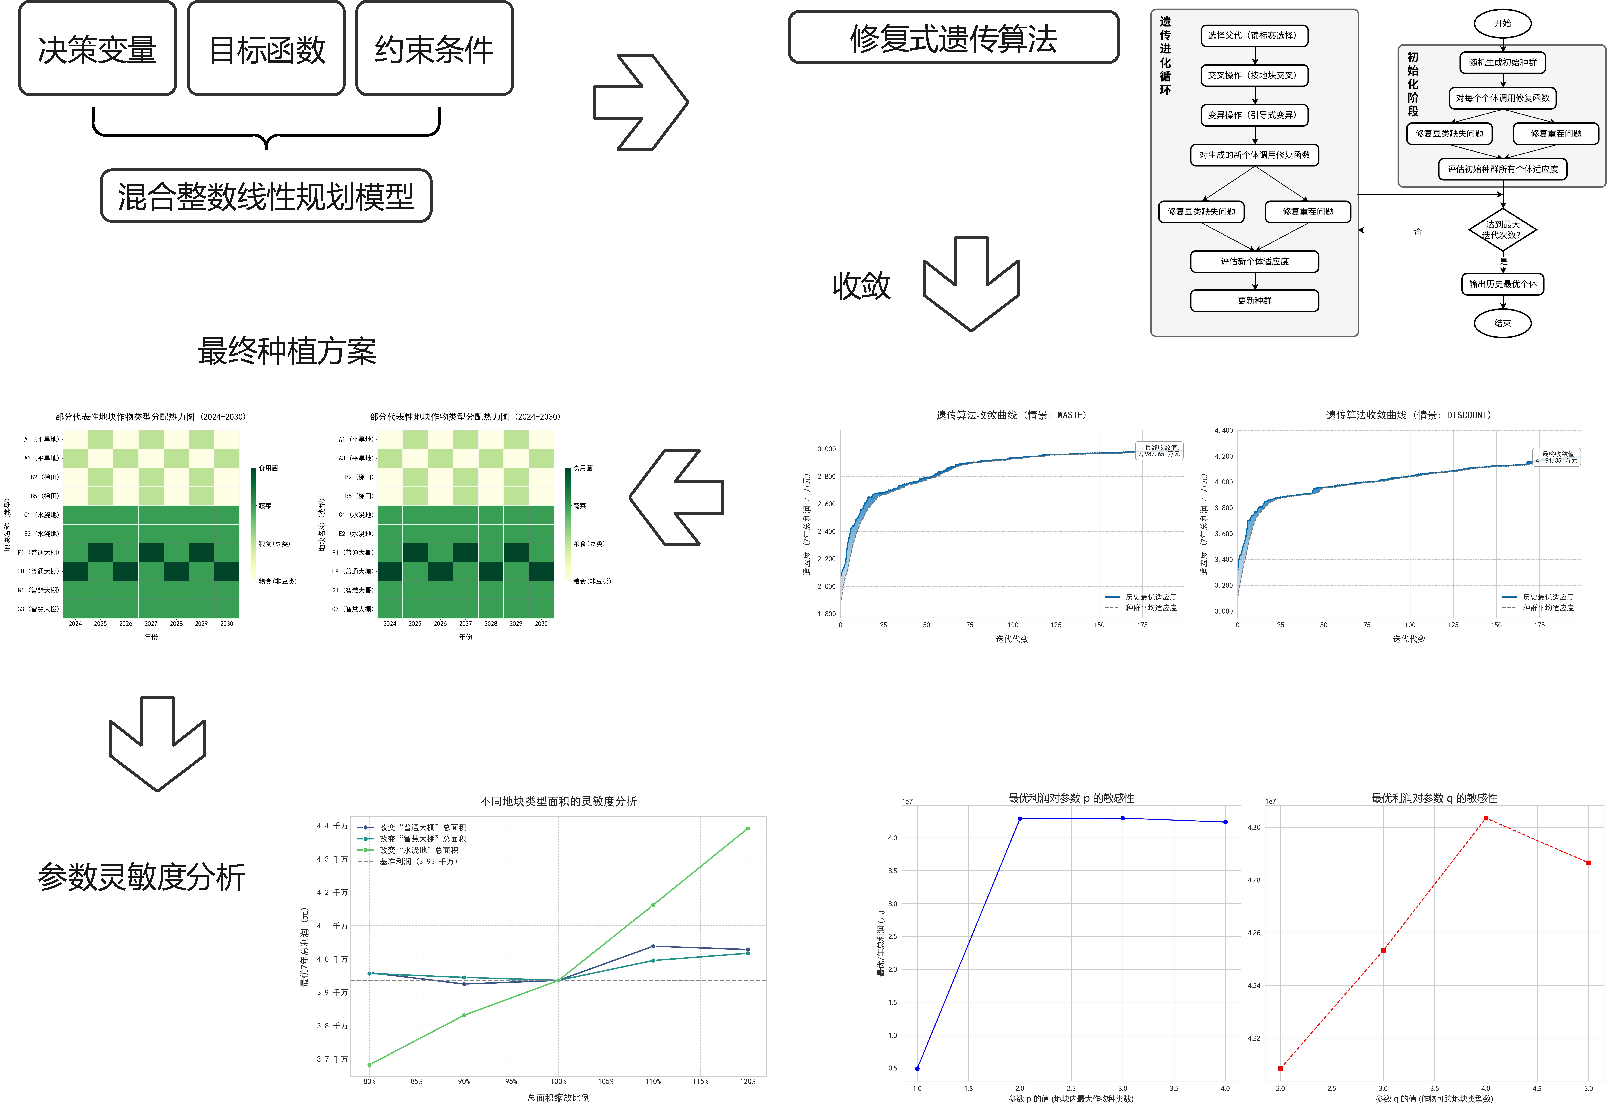
\includegraphics[width=0.8\textwidth]{figs/3问题一/问题一框架.pdf}
    \caption{问题一的混合整数线性规划模型概念框架图。}
    \label{fig:milp_framework}
\end{figure}

\subsection{模型构建}


为将该乡村的长期种植规划问题转化为一个可求解的数学模型,我们构建了一个多周期混合整数线性规划(MILP)模型。该模型以古典微观经济学中的厂商理论为基础,将乡村视为一个追求长期利润最大化的理性决策主体。模型的构建过程遵循模块化原则,依次定义了决策变量、目标函数和约束条件三个核心部分。

\subsubsection{决策变量}

模型的决策核心在于如何在给定的时间和空间维度上分配种植资源。为此,我们定义了以下四组核心决策变量,它们共同构成了完整的七年种植方案:
\begin{itemize}
    \item $a_{ijky}$: 一个连续变量,表示在年份 $y$ 的第 $k$ 季,于地块 $i$ 上种植作物 $j$ 的面积(亩)。
    \item $x_{ijky}$: 一个二进制变量,当 $a_{ijky} > 0$ 时为1,否则为0。它表示是否在年份 $y$ 的第 $k$ 季,于地块 $i$ 上安排种植作物 $j$。
    \item $\text{normal}_{jy}$: 一个连续辅助变量,表示年份 $y$ 作物 $j$ 未超出预期销售量的产量部分(斤)。
    \item $\text{over}_{jy}$: 一个连续辅助变量,表示年份 $y$ 作物 $j$ 超出预期销售量的产量部分(斤)。
\end{itemize}



\subsubsection{目标函数}

模型的总体目标是最大化2024年至2030年这七年间的累计总利润。总利润定义为总销售收入与总种植成本的差额。总种植成本的计算公式为:
\begin{equation}
\text{Cost} = \sum_{y \in Y} \sum_{i \in I} \sum_{j \in J} \sum_{k \in K} a_{ijky} \cdot C_{jy}
\end{equation}
根据题目要求,针对超出预期销售量的农产品处置方式,分别构建了两种情景下的目标函数。

\textbf{情景 1:超出部分滞销}

在此情景下,任何超出预期销售量的产品均无市场价值,总收入仅来源于正常销售部分。因此,目标函数 $Z_1$ 定义为:
\begin{equation}
\text{Maximize} \quad Z_1 = \sum_{y \in Y} \sum_{j \in J} (\text{normal}_{jy} \cdot P_{jy}) - \text{Cost}
\end{equation}

\textbf{情景 2:超出部分降价出售}

在此情景下,超出预期销售量的产品可以按正常价格的50\%进行销售,从而产生额外收入。因此,目标函数 $Z_2$ 定义为:
\begin{equation}
\text{Maximize} \quad Z_2 = \sum_{y \in Y} \sum_{j \in J} (\text{normal}_{jy} \cdot P_{jy} + \text{over}_{jy} \cdot (0.5 \cdot P_{jy})) - \text{Cost}
\end{equation}

\subsubsection{约束条件}

为确保种植方案在现实中可实施、在农艺上合理、在生态上可持续,我们建立了系统的约束集。该约束覆盖土地、劳动力、用水与设施容量等物理资源上限。包含种植制度、轮作间隔与病虫害防控等农艺要求。纳入产销平衡、价格与合同约束、库存与流通能力等市场规则。加入土壤养分恢复、水资源红线与排放限额等长期生态限制。上述约束以可检验的数学形式(线性不等式与逻辑条件)进入模型,并在求解过程中严格满足。

\textbf{1. 总产量与销售部分关联}

为建立生产与市场销售之间的平衡关系,任何一种作物的年总产量必须等于其正常销售量与超预期销售量之和。同时,其正常销售部分的产量不能突破市场的预期销售量上限。
\begin{gather}
\sum_{i \in I} \sum_{k \in K} a_{ijky} \cdot \text{yield}_{jy} = \text{normal}_{jy} + \text{over}_{jy} \quad (\forall j \in J, y \in Y) \label{eq:yield_balance} \\
\text{normal}_{jy} \le \text{sale}_{jy} \quad (\forall j \in J, y \in Y) \label{eq:normal_sale_limit}
\end{gather}
此外,所有与面积和产量相关的变量均需满足非负性。
\begin{equation}
a_{ijky}, \text{normal}_{jy}, \text{over}_{jy} \ge 0 \label{eq:non_negativity}
\end{equation}

\textbf{2. 决策变量关联}

为确保二进制决策变量 $x_{ijky}$ 与连续决策变量 $a_{ijky}$ 的逻辑一致性,即仅当决定进行某项种植活动时 ($x_{ijky}=1$),相应的种植面积 ($a_{ijky}$) 才可为正,引入以下约束。其中,$M$ 是一个足够大的正数,$\epsilon$ 是一个极小的正数,用以规定最小种植阈值。
\begin{gather}
a_{ijky} \le M \cdot x_{ijky} \quad (\forall i, j, k, y) \label{eq:big_m} \\
a_{ijky} \ge \epsilon \cdot x_{ijky} \quad (\forall i, j, k, y) \label{eq:min_area}
\end{gather}

\textbf{3. 土地适宜性约束}

农作物的生长对其环境有特定要求,因此任何种植安排都必须遵循农作物对土地类型和季节的适应性。
\begin{equation}
x_{ijky} \le S_{ijk} \quad (\forall i, j, k, y) \label{eq:suitability}
\end{equation}

\textbf{4. 地块面积约束}

任何地块在任一季节内,所有作物的种植面积之和不能超过该地块的物理总面积。
\begin{equation}
\sum_{j \in J} a_{ijky} \le A_i \quad (\forall i \in I, k \in K, y \in Y) \label{eq:area_limit}
\end{equation}

\textbf{5. 重茬约束}

为了维护土壤健康和防止产量下降,模型禁止在同一地块连续两年种植同一种作物。该农艺规则通过引入辅助二进制变量 $z_{ijy}$ 来实现,该变量用以标记作物 $j$ 在年份 $y$ 是否在地块 $i$ 上种植过。
\begin{gather}
z_{ijy} \ge x_{ijky} \quad (\forall i, j, k, y) \label{eq:z_def1} \\
\sum_{k \in K} x_{ijky} \ge z_{ijy} \quad (\forall i, j, y) \label{eq:z_def2} \\
z_{ijy} + z_{ij,y-1} \le 1 \quad (\forall i, j, y) \label{eq:rotation}
\end{gather}
对于规划的起始年份2024年,此约束需与2023年的种植历史数据 $H_{ij,2023}$ 进行衔接。
\begin{equation}
z_{ij,2024} + H_{ij,2023} \le 1 \quad (\forall i, j) \label{eq:rotation_init}
\end{equation}

\textbf{6. 豆类种植约束}

基于豆类作物能够固氮改良土壤的特性,规定所有地块在任意连续三年周期内,必须至少安排一次豆类作物的种植。
\begin{equation}
\sum_{j \in J_{\text{legume}}} (z_{ij,y} + z_{ij,y+1} + z_{ij,y+2}) \ge 1 \quad (\forall i, y \in \{2024, \dots, 2028\}) \label{eq:legume}
\end{equation}
此约束的初始条件也需要结合2022年和2023年的历史种植数据进行调整,以保证规则的完整性。

\textbf{7. 分散性约束}

为提高耕作效率和方便田间管理,对种植方案的作物分布施加限制。首先,在同一季节,每个地块内种植的作物种类不应超过预设上限 $p$。
\begin{equation}
\sum_{j \in J} x_{ijky} \le p \quad (\forall i, k, y) \label{eq:p_limit}
\end{equation}
其次,为避免单一作物过于分散地种植,规定在同一季节,每种作物允许种植的地块类型数量不应超过预设上限 $q$。此约束通过引入辅助二进制变量 $w_{jtky}$ 实现,该变量标记作物 $j$ 是否在年份 $y$ 的 $k$ 季种植于类型为 $t$ 的土地上。
\begin{gather}
x_{ijky} \le w_{jtky} \quad \text{where } t = \text{Type}(i) \quad (\forall i, j, k, y) \label{eq:w_def1} \\
\sum_{i \in I, \text{Type}(i)=t} x_{ijky} \ge w_{jtky} \quad (\forall j, t, k, y) \label{eq:w_def2} \\
\sum_{t \in T} w_{jtky} \le q \quad (\forall j, k, y) \label{eq:q_limit}
\end{gather}







\subsubsection{优化模型的整合呈现}

基于前文对各组成要素的定义,现给出混合整数线性规划模型的完整表述。该表述包含决策变量、目标函数,以及关于市场、土地、农艺与管理的全部约束。由此形成用于求解最优种植方案的数学框架。模型的总目标为最大化总利润$Z$。针对题目中超售产品处置的两种情景,$Z$的计算公式分别定义如下:
\begin{itemize}
    \item \textbf{情景 1 (滞销):} $Z = \sum_{y \in Y} \sum_{j \in J} (\text{normal}_{jy} \cdot P_{jy}) - \text{Cost}$
    \item \textbf{情景 2 (降价出售):} $Z = \sum_{y \in Y} \sum_{j \in J} (\text{normal}_{jy} \cdot P_{jy} + \text{over}_{jy} \cdot (0.5 \cdot P_{jy})) - \text{Cost}$
\end{itemize}
其中,总成本 $\text{Cost} = \sum_{y \in Y} \sum_{i \in I} \sum_{j \in J} \sum_{k \in K} a_{ijky} \cdot C_{jy}$。

完整的优化模型表述为:
\begin{flalign}
    \text{Maximize} \quad & Z & \\
    \text{subject to} \quad & \sum_{i \in I} \sum_{k \in K} a_{ijky} \cdot \text{yield}_{jy} = \text{normal}_{jy} + \text{over}_{jy} & \forall j, y \label{con:yield_balance} \\
    & \text{normal}_{jy} \le \text{sale}_{jy} & \forall j, y \label{con:normal_sale_limit} \\
    & a_{ijky} \le M \cdot x_{ijky} & \forall i, j, k, y \label{con:big_m} \\
    & a_{ijky} \ge \epsilon \cdot x_{ijky} & \forall i, j, k, y \label{con:min_area} \\
    & x_{ijky} \le S_{ijk} & \forall i, j, k, y \label{con:suitability} \\
    & \sum_{j \in J} a_{ijky} \le A_i & \forall i, k, y \label{con:area_limit} \\
    & z_{ijy} \ge x_{ijky} & \forall i, j, k, y \label{con:z_def1} \\
    & \sum_{k \in K} x_{ijky} \ge z_{ijy} & \forall i, j, y \label{con:z_def2} \\
    & z_{ijy} + z_{ij,y-1} \le 1 & \forall i, j, y \label{con:rotation} \\
    & z_{ij,2024} + H_{ij,2023} \le 1 & \forall i, j \label{con:rotation_init} \\
    & \sum_{j \in J_{\text{legume}}} (z_{ij,y} + z_{ij,y+1} + z_{ij,y+2}) \ge 1 & \forall i, y \in \{2024, \dots, 2028\} \label{con:legume} \\
    & \sum_{j \in J} x_{ijky} \le p & \forall i, k, y \label{con:p_limit} \\
    & x_{ijky} \le w_{jtky}, \quad t = \text{Type}(i) & \forall i, j, k, y \label{con:w_def1} \\
    & \sum_{i \in I, \text{Type}(i)=t} x_{ijky} \ge w_{jtky} & \forall j, t, k, y \label{con:w_def2} \\
    & \sum_{t \in T} w_{jtky} \le q & \forall j, k, y \label{con:q_limit} \\
    & a_{ijky}, \text{normal}_{jy}, \text{over}_{jy} \ge 0 & \forall i, j, k, y \label{con:non_negativity} \\
    & x_{ijky}, z_{ijy}, w_{jtky} \in \{0, 1\} & \forall i, j, t, k, y \label{con:binary}
\end{flalign}


\subsection{模型求解与算法设计}

前文构建的混合整数线性规划模型,因其决策变量众多、约束条件复杂且相互交织,构成了一个典型的NP-Hard组合优化问题。该问题的解空间随着规划年限和地块数量的增加而呈指数级增长,导致传统的精确求解方法,如穷举搜索,在计算上是不可行的。尽管商业或开源的精确求解器(如CBC、Gurobi)理论上能够找到全局最优解,但在面对如此大规模的实例时,其求解时间往往难以接受,且建模过程相对繁琐。因此,为了在有限时间内获得高质量的可行解,本文设计并实现了一种启发式算法进行求解,其框架如图\ref{fig:algorithm_framework}所示。

\begin{figure}[htbp]
    \centering
    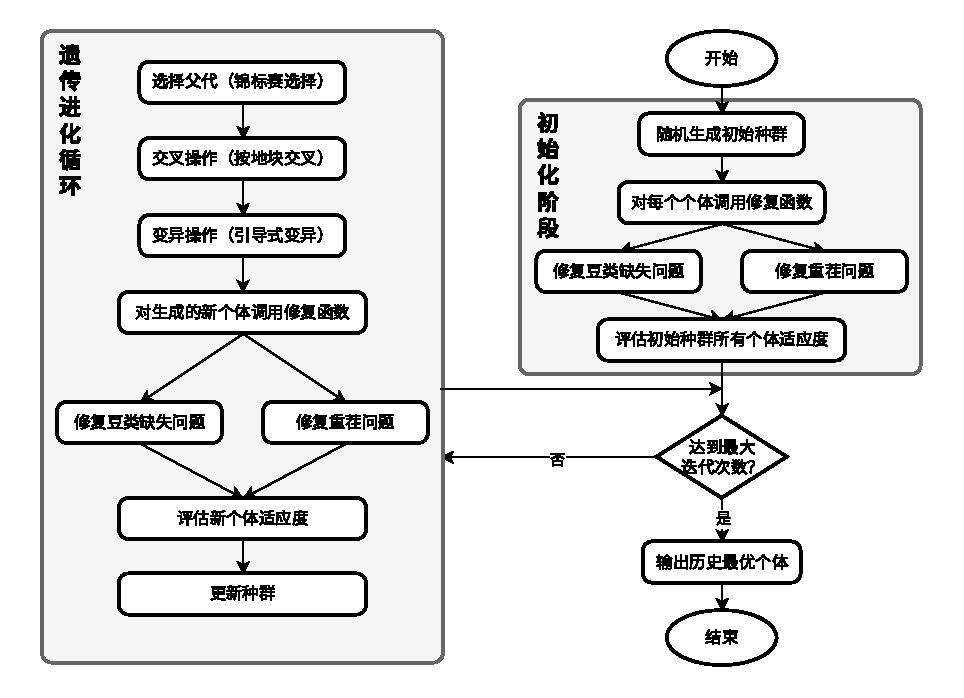
\includegraphics[width=0.9\textwidth]{figs/3问题一/遗传算法图.pdf}
    \caption{修复式遗传算法框架}
    \label{fig:algorithm_framework}
\end{figure}


\subsubsection{算法选择与基本原理}

在算法选型阶段,我们评估了多种方案。初步尝试的基础遗传算法依赖于惩罚函数来处理约束,但实践表明,由于本模型存在大量严格的“硬”约束(例如重茬和豆类轮作),随机生成的初始解几乎全部违反约束。这导致适应度函数被巨大的惩罚项主导,使得算法难以在广阔的不可行域中有效搜索,收敛性能不佳。

为了克服这一挑战,我们最终选择采用一种\textbf{修复式遗传算法}。该方法的核心思想是将领域知识,即模型的各项约束规则,内嵌到一个确定性的“修复函数”中。遗传算法强大的全局搜索能力得以保留,同时通过修复机制保证了在进化的每一个环节(包括种群初始化、交叉和变异之后),所有个体都始终是满足核心约束的可行解。这种设计将算法的搜索焦点从“如何避免违反约束”转移到“如何在可行域内寻找更优解”,从而显著净化了搜索空间,极大地提升了算法的收敛效率和稳定性。

\subsubsection{修复式遗传算法实现细节}

\textbf{解决方案编码}

为了直观地表示一个完整的七年种植计划,我们采用结构化的字典对染色体进行编码。其基本格式为:{年份: {季节: {地块名称: 作物名称}}}。例如,一个个体中的\text{solution[2025][1]['A1']} = '玉米',明确表示2025年第一季在A1地块种植玉米。此编码方式不仅便于理解,也为后续的遗传算子操作提供了便利。

\textbf{适应度函数}

适应度函数直接定义为问题所追求的七年总利润,其计算方式与目标函数一致。根据两种不同的市场情景(超出部分滞销或折价出售),我们实现了相应的收入计算逻辑。由于所有核心约束均由修复函数处理,适应度函数中不包含任何惩罚项,确保了其评估的纯粹性,即直接反映解的经济效益。

\textbf{修复函数}

修复函数是本算法的关键所在,它在种群初始化以及每次交叉和变异操作后被调用,以确保所有个体始终满足农艺要求。该函数主要执行两项修复任务:
\begin{itemize}
    \item 修复重茬问题:算法会遍历方案中的所有地块和年份,检查是否存在与前一年种植相同作物的情况。一旦发现重茬,系统将从一个预先定义的、不包含前一年作物的合法候选作物列表中,随机选择一种进行替换。
    \item 修复豆类缺失问题: 算法会遍历所有地块的每一个三年窗口期(起始于2023年)。若发现某个窗口期内未能满足至少种植一次豆类作物的要求,系统将强制在该窗口期内的某一年随机选择一个季节,将原定作物替换为一种合法的、且不与前一年构成重茬的豆类作物。
\end{itemize}

\textbf{遗传算子}

\begin{itemize}
    \item \textbf{选择:} 采用经典的锦标赛选择机制。每次从种群中随机选择$k$个个体(本文设$k=3$),并将其中适应度最高的个体选入下一代种群的父代池。
    \item \textbf{交叉:} 设计了按地块交叉的策略。以一定的交叉概率,随机选择若干地块,然后交换两个父代个体在这些选定地块上的完整七年种植历史,从而生成子代。
    \item \textbf{变异:} 采用引导式变异。随机选择方案中的若干基因位点(即某个地块在某年某季的种植决策),并从一个预先筛选好的、针对该地块和季节的“合法作物列表”中随机选择一种新作物进行替换。这种方式保证了变异操作本身不会引入明显不合理的种植安排。
\end{itemize}

\textbf{主要超参数设置}

通过多次调试与实验,我们为算法设定了一组表现良好的关键超参数,具体如下:种群大小为100,最大迭代代数为200,交叉概率为0.8,变异概率为0.2。


\subsection{求解结果与分析}

基于上述模型与算法,我们分别对情景一(超出部分滞销)和情景二(超出部分降价出售)进行了求解。本节将展示算法的收敛性能、最优种植方案的构成以及各类作物的具体产量安排。

\subsubsection{算法收敛性分析}


为了验证修复式遗传算法的有效性,我们追踪并记录了其在200次迭代过程中的适应度变化。如图\ref{fig:convergence}所示,横轴为进化代数,纵轴为七年总利润。图中展示了每一代种群的历史最优适应度与平均适应度。

在两种情景下,最优适应度曲线快速上升,并分别收敛于2987.65万元与4191.35万元。这表明算法能在有限迭代内找到高质量解。平均适应度曲线平稳增长。两条曲线在后期逐渐趋近,说明种群整体向最优解集中,形成稳定收敛。

\begin{figure}[H]
    \centering
    \begin{subfigure}[b]{0.48\textwidth}
        \centering
        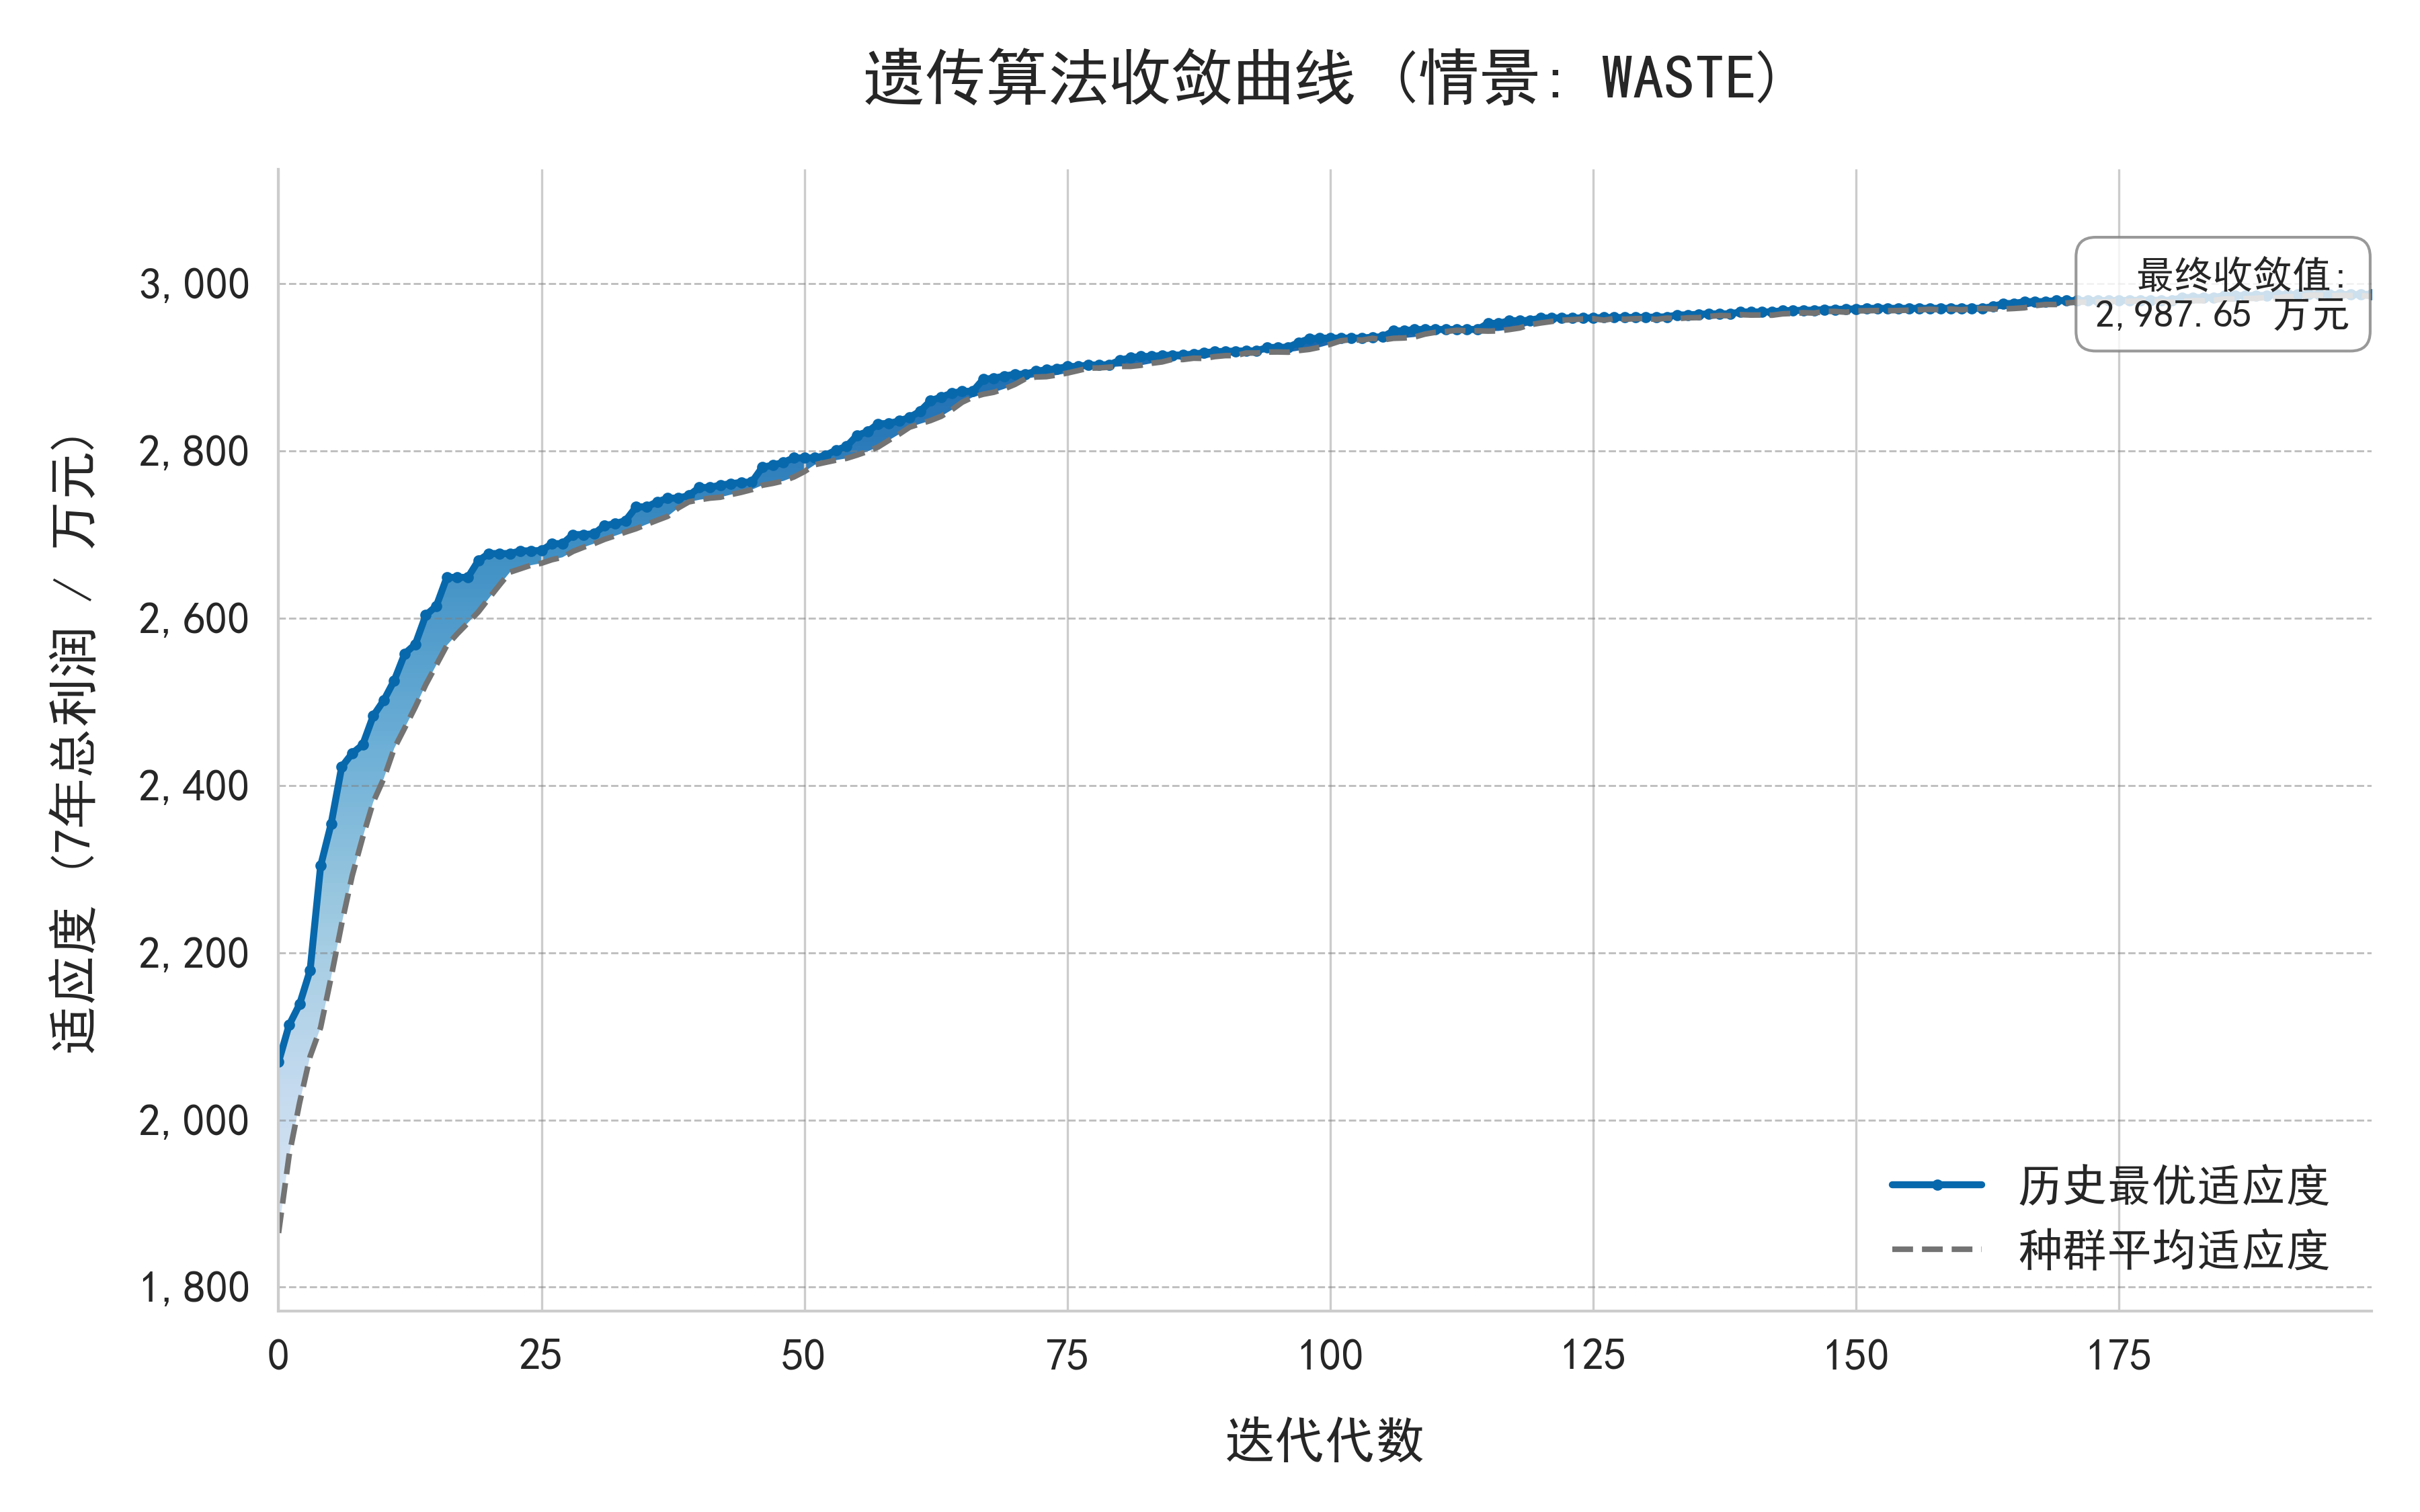
\includegraphics[width=\textwidth]{figs/3问题一/情况一ga训练曲线.png}
        \caption{情景一(超出部分滞销)收敛过程}
        \label{fig:conv_case1}
    \end{subfigure}
    \hfill
    \begin{subfigure}[b]{0.48\textwidth}
        \centering
        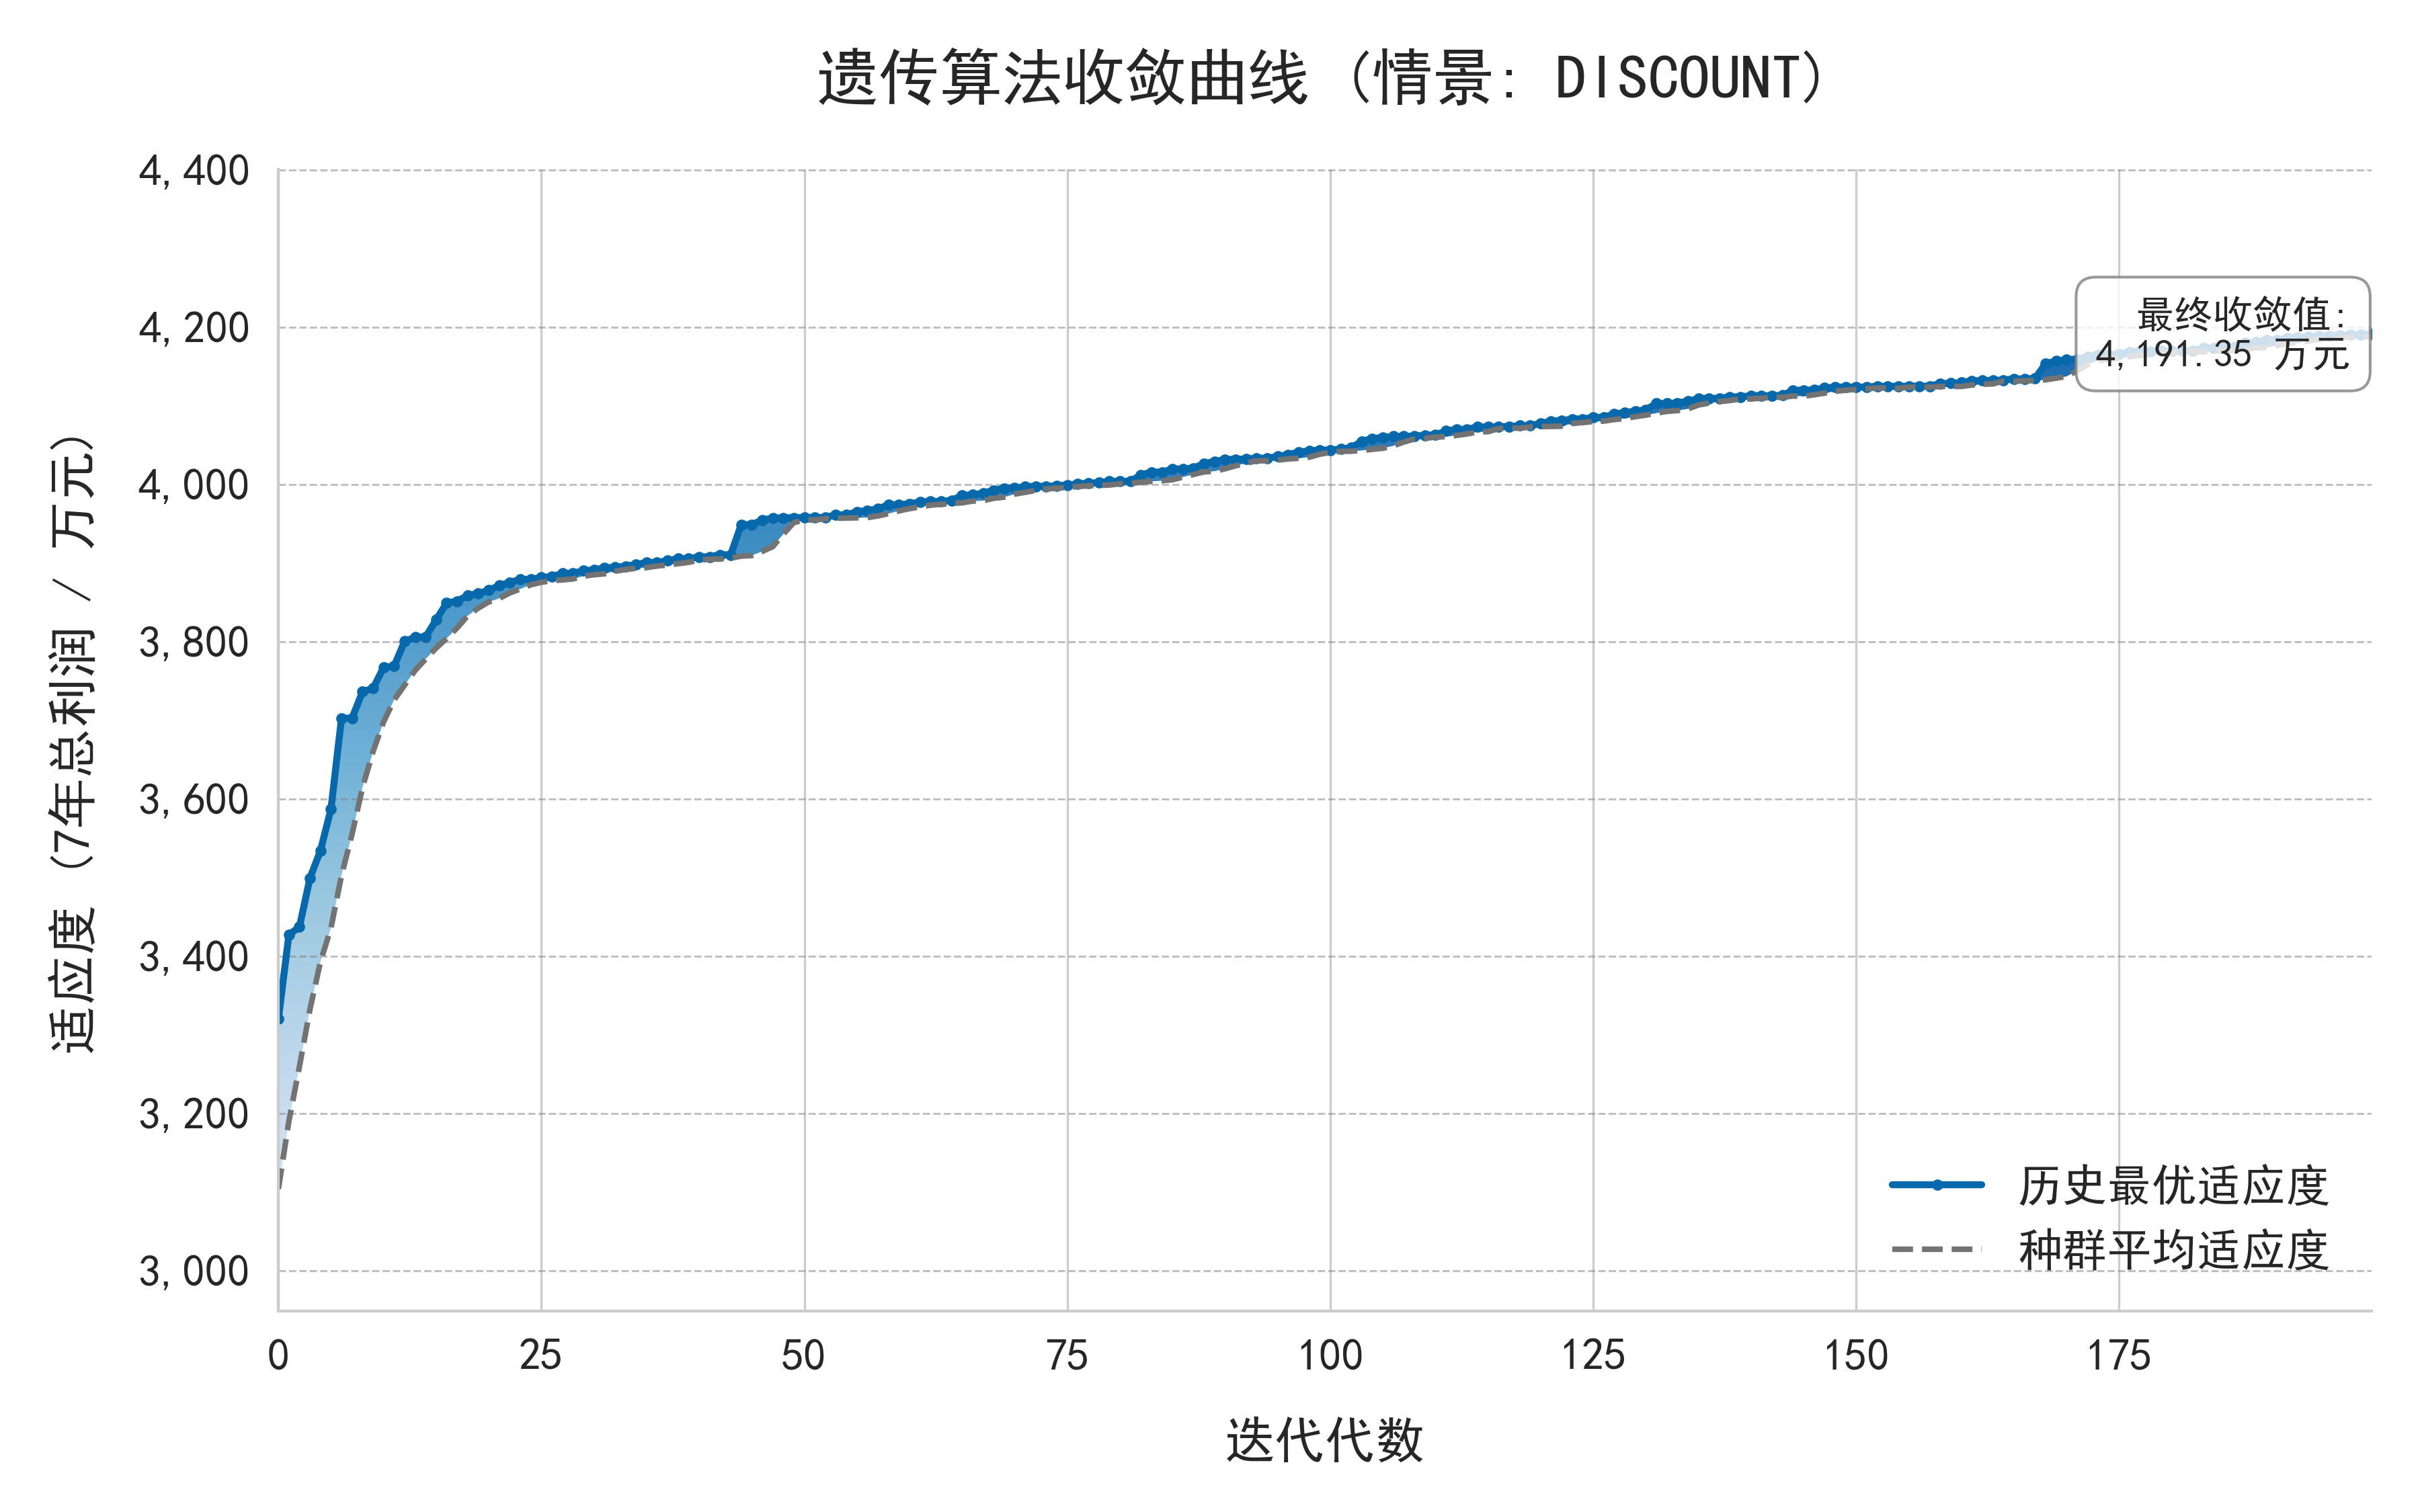
\includegraphics[width=\textwidth]{figs/3问题一/情况二ga训练曲线.png}
        \caption{情景二(超出部分降价)收敛过程}
        \label{fig:conv_case2}
    \end{subfigure}
    \caption{两种情景下修复式遗传算法的适应度收敛曲线。}
    \label{fig:convergence}
\end{figure}

\subsubsection{最优种植方案}
算法求解得到的最优七年种植方案细节繁多,为了直观地展示其时空分布特性,我们采用热力图进行可视化,如图\ref{fig:heatmap}所示。热力图的纵轴代表34个露天耕地地块和20个大棚,横轴为2024至2030年。图中不同颜色对应不同的农作物,清晰地展示了各项作物在不同地块间的轮作模式。

从图中可以观察到,高价值作物(如蔬菜、食用菌)优先被分配到生产效率更高的大棚和水浇地。同时,豆类作物(如大豆)的种植被周期性地安排在各地块中,严格满足了三年至少种植一次的农艺要求。整体方案在空间上呈现出一定的聚集性,有利于规模化管理。

\begin{figure}[H]
    \centering
    \begin{subfigure}[b]{0.8\textwidth}
        \centering
        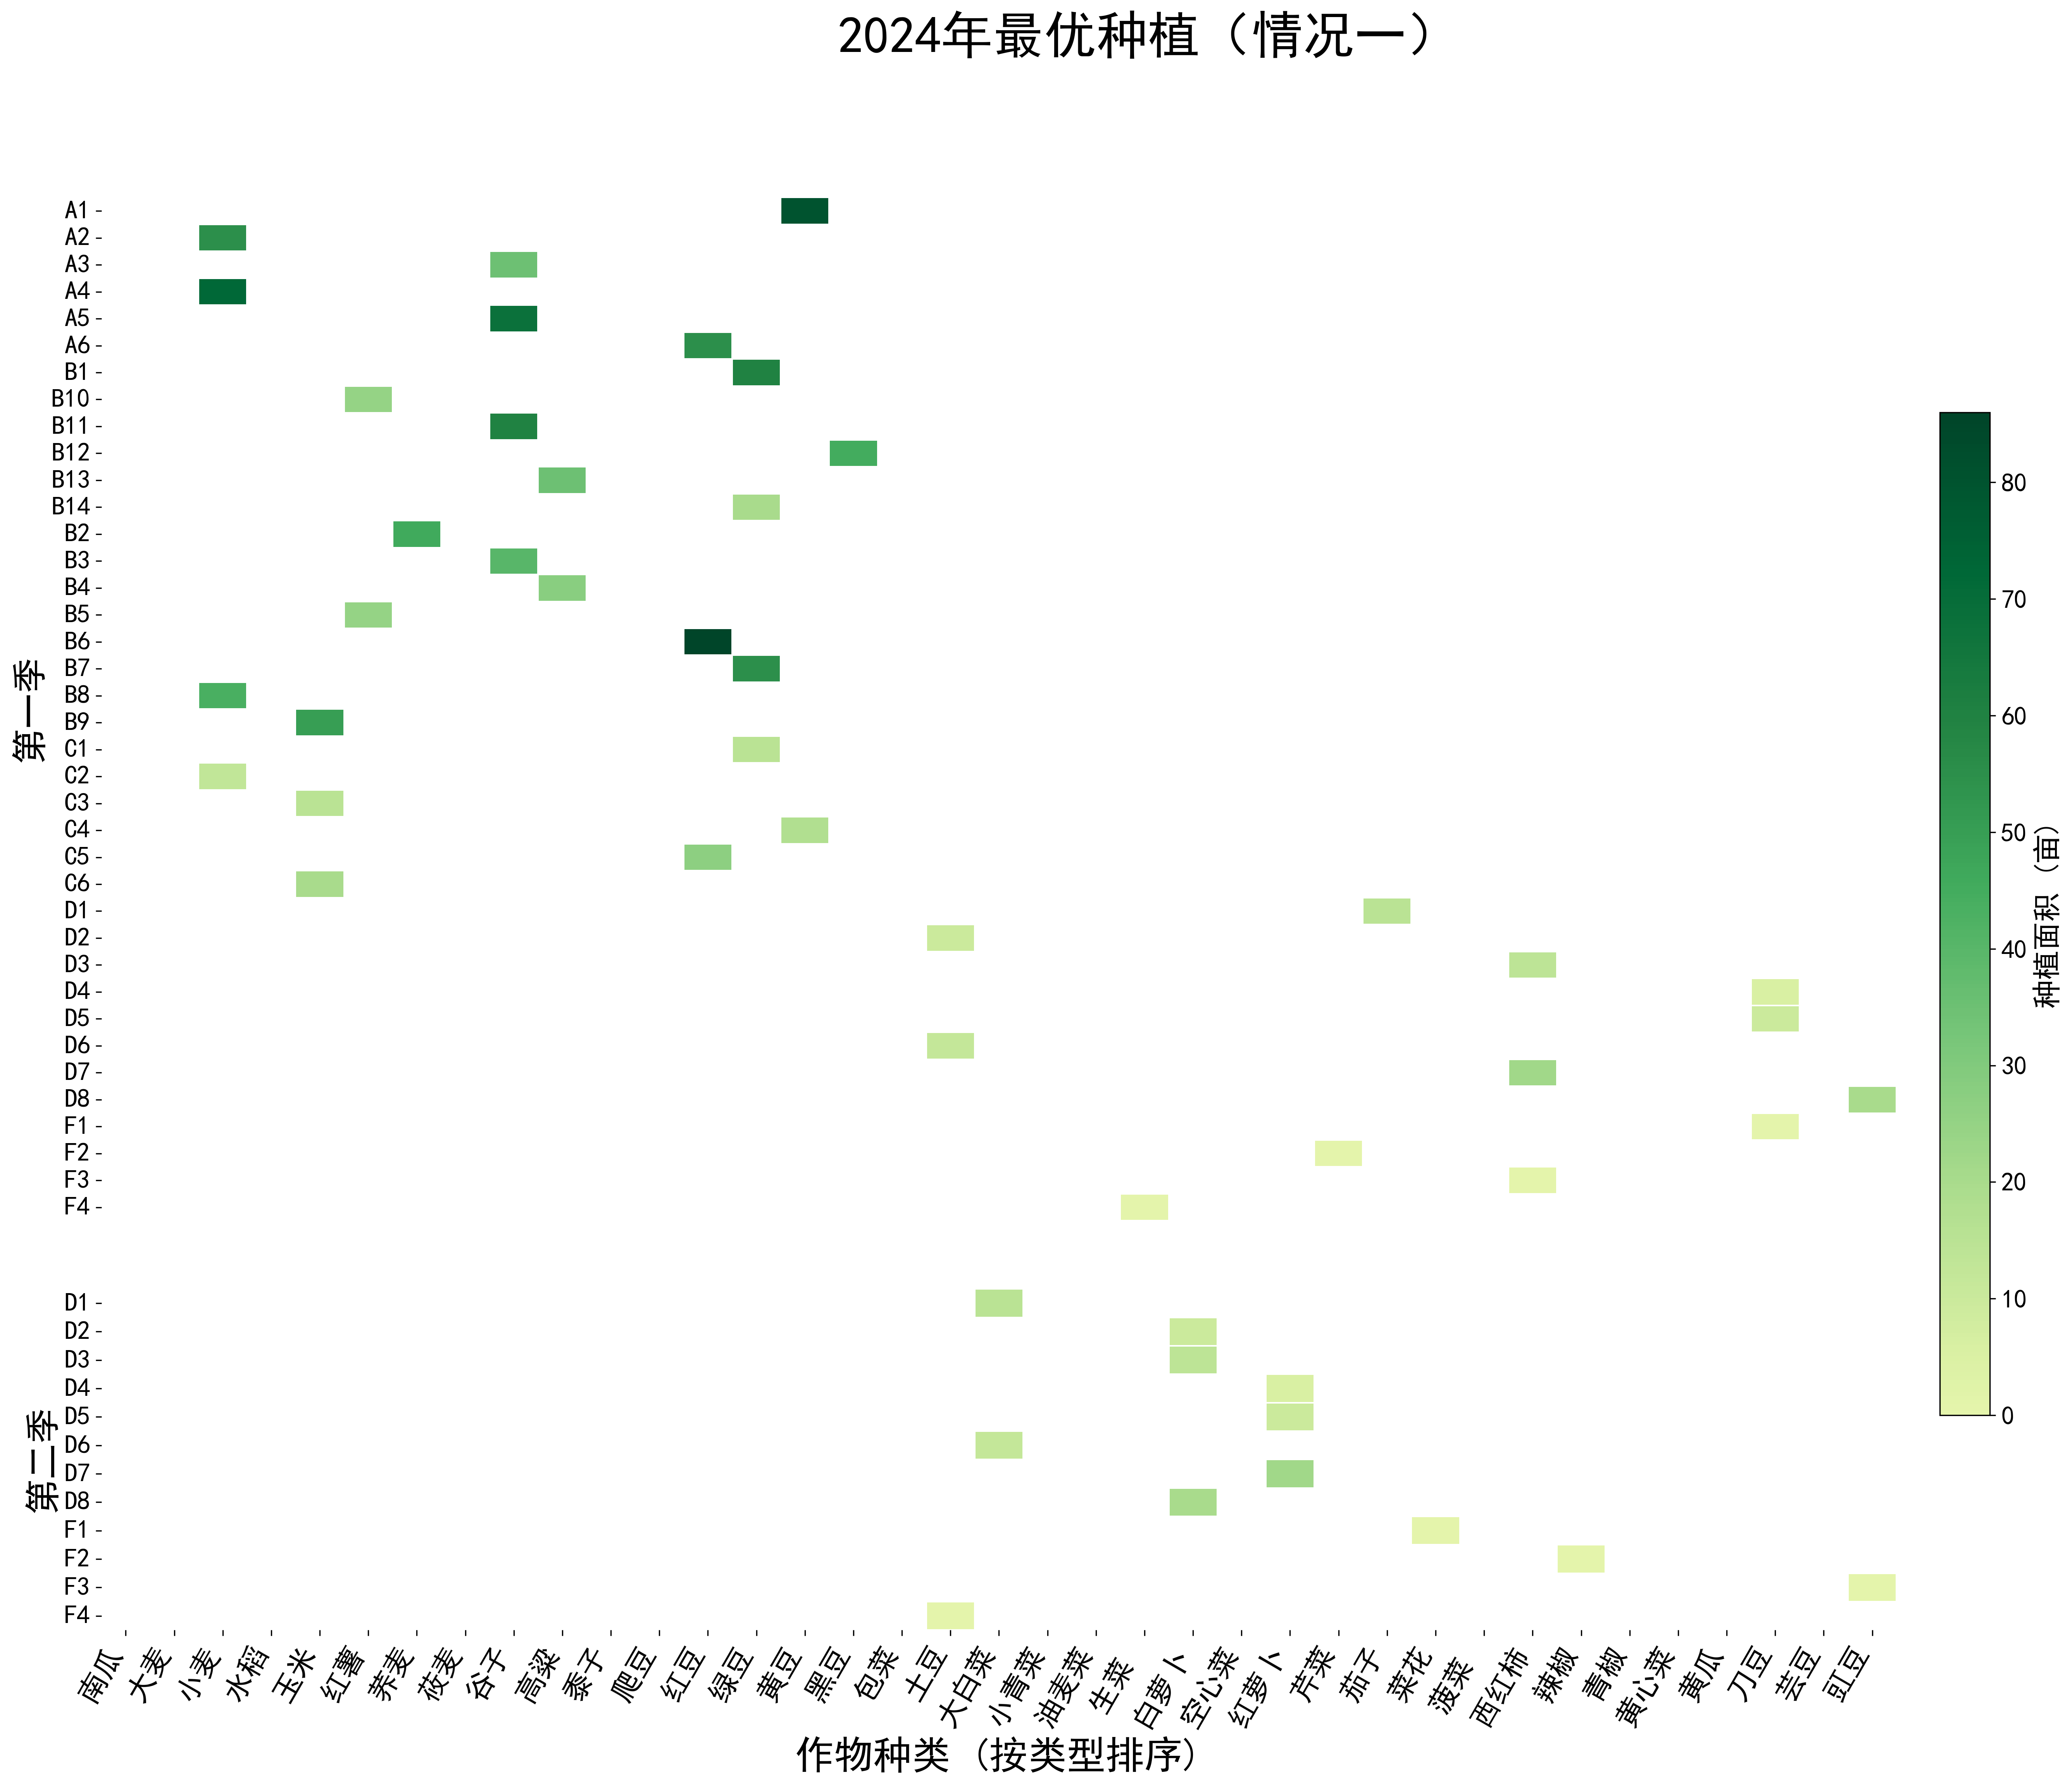
\includegraphics[width=\textwidth]{figs/3问题一/2024年最优种植方案(情况一).png}
        \caption{情景一(超出部分滞销)最优种植方案}
        \label{fig:heatmap_case1}
    \end{subfigure}
    \vfill
    \begin{subfigure}[b]{0.8\textwidth}
        \centering
        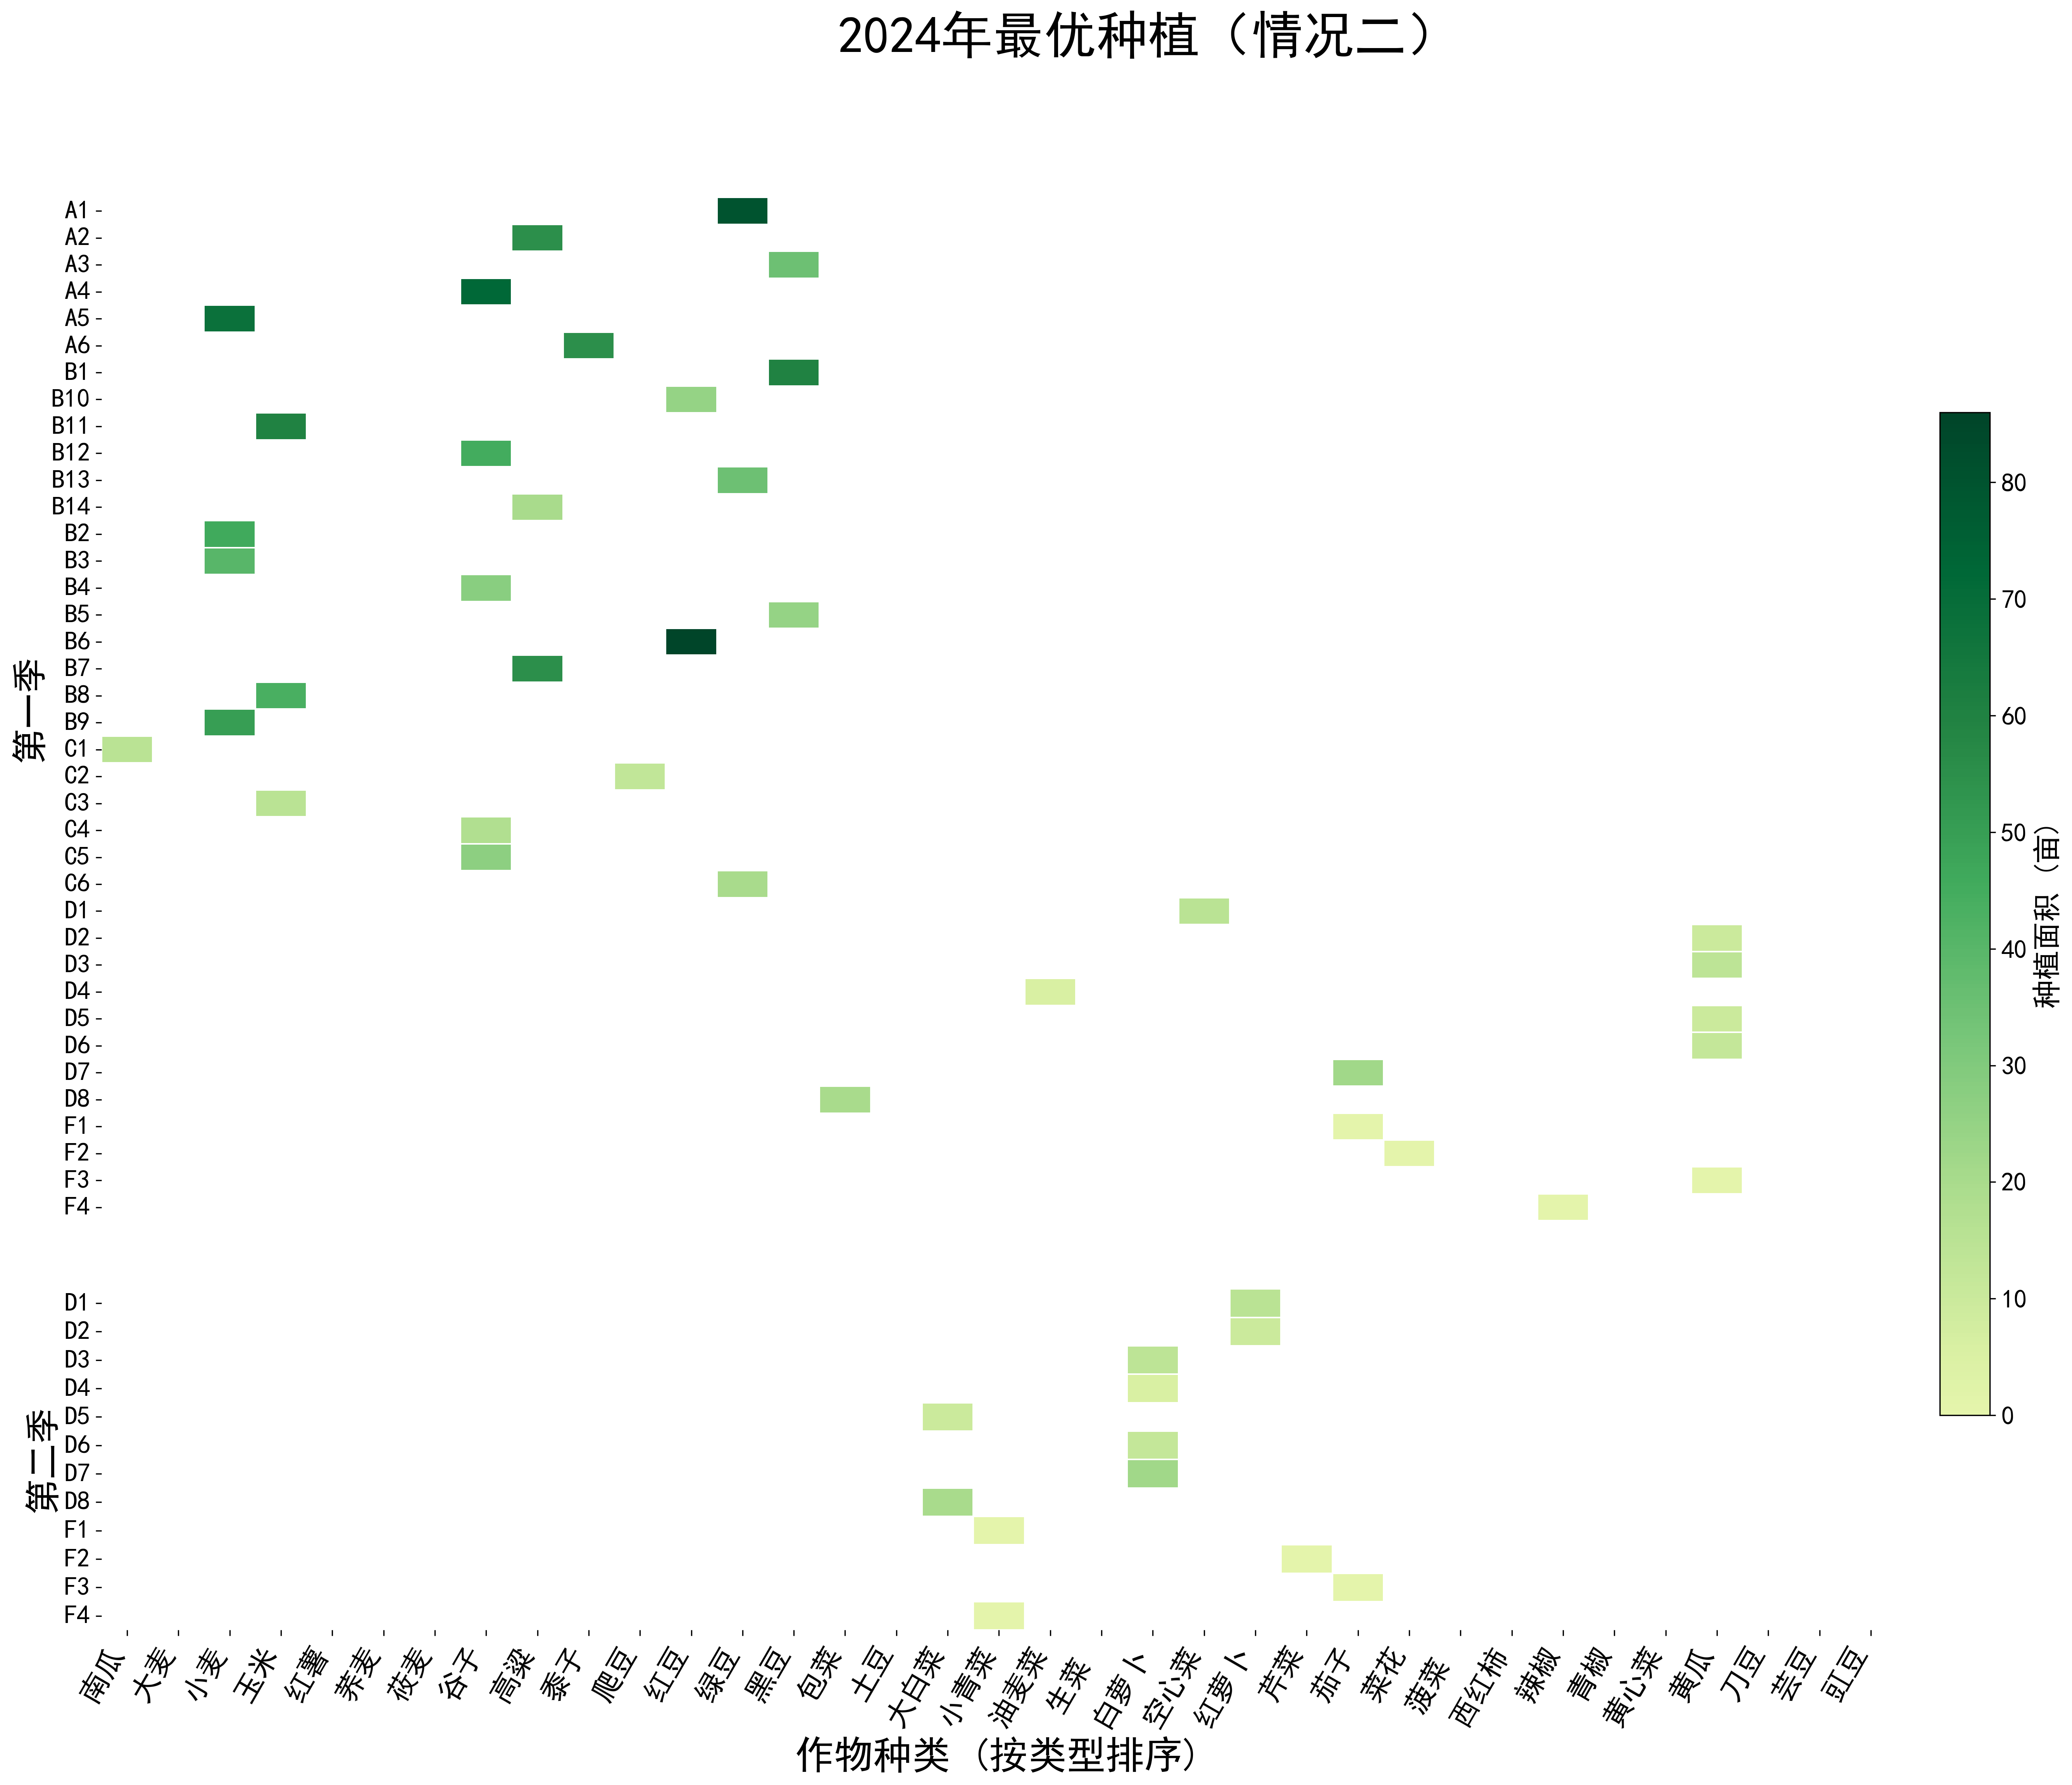
\includegraphics[width=\textwidth]{figs/3问题一/2024年最优种植方案(情况二).png}

        \caption{情景二(超出部分降价)最优种植方案}
        \label{fig:heatmap_case2}
    \end{subfigure}
    \caption{两种情景下2024-2030年最优种植方案时空分布热力图。}
    \label{fig:heatmap}
\end{figure}



\subsection{灵敏度分析}

为了探究模型最优解对关键参数变化的响应程度,并验证结果的稳健性,我们进行了多维度灵敏度分析。分析的核心方法是采用“一次单因素变动(One-at-a-Time, OAT)”,即在保持其他参数为基准值不变的条件下,系统性地调整某一个特定参数,并重新运行完整的优化过程,观察最优总利润的变化。本节将重点分析管理便利性参数与关键土地资源面积这两个维度的影响。

\subsubsection{管理便利性参数p与q的灵敏度分析}

参数 $p$(地块内允许种植的作物种类上限)和 $q$(一种作物允许种植的地块类型数量上限)是为保证田间管理便利性而引入的重要约束。我们通过改变这两个参数的取值,探究了其对最优七年总利润的影响,结果如图\ref{fig:pq_sensitivity}所示。

分析左图可知,总利润对参数 $p$ 的变化表现出极高的敏感性,尤其是在 $p$ 从1增加到2的区间。当 $p=1$ 时,每个地块在每个季节只能种植一种作物,这种严格的单一种植模式极大地限制了轮作和作物搭配的灵活性,导致总利润仅为约500万元。当 $p$ 放宽至2时,总利润跃升至超过4000万元,实现了数量级的增长。这表明允许地块内进行适度的作物组合是实现高利润的必要条件。当 $p$ 继续增加到3和4时,总利润的增长趋于平缓,说明 $p=2$ 已经释放了模型绝大部分的优化潜力。

分析右图可知,总利润随参数 $q$ 的增加而呈现清晰的上升趋势,并在 $q=4$ 时达到峰值,约为4310万元。这说明,允许一种作物被种植在更多不同类型的地块上,能为模型提供更大的决策自由度,从而更有效地利用各类土地资源以实现利润最大化。当 $q$ 从4增加到5时,利润出现轻微回落,这可能意味着过度的分散性不再带来边际效益,甚至可能因为启发式算法的搜索特性,在更复杂的解空间中未能收敛到更好的解。综合来看,$q=4$ 是本模型的一个较优配置。

\begin{figure}[H]
    \centering
    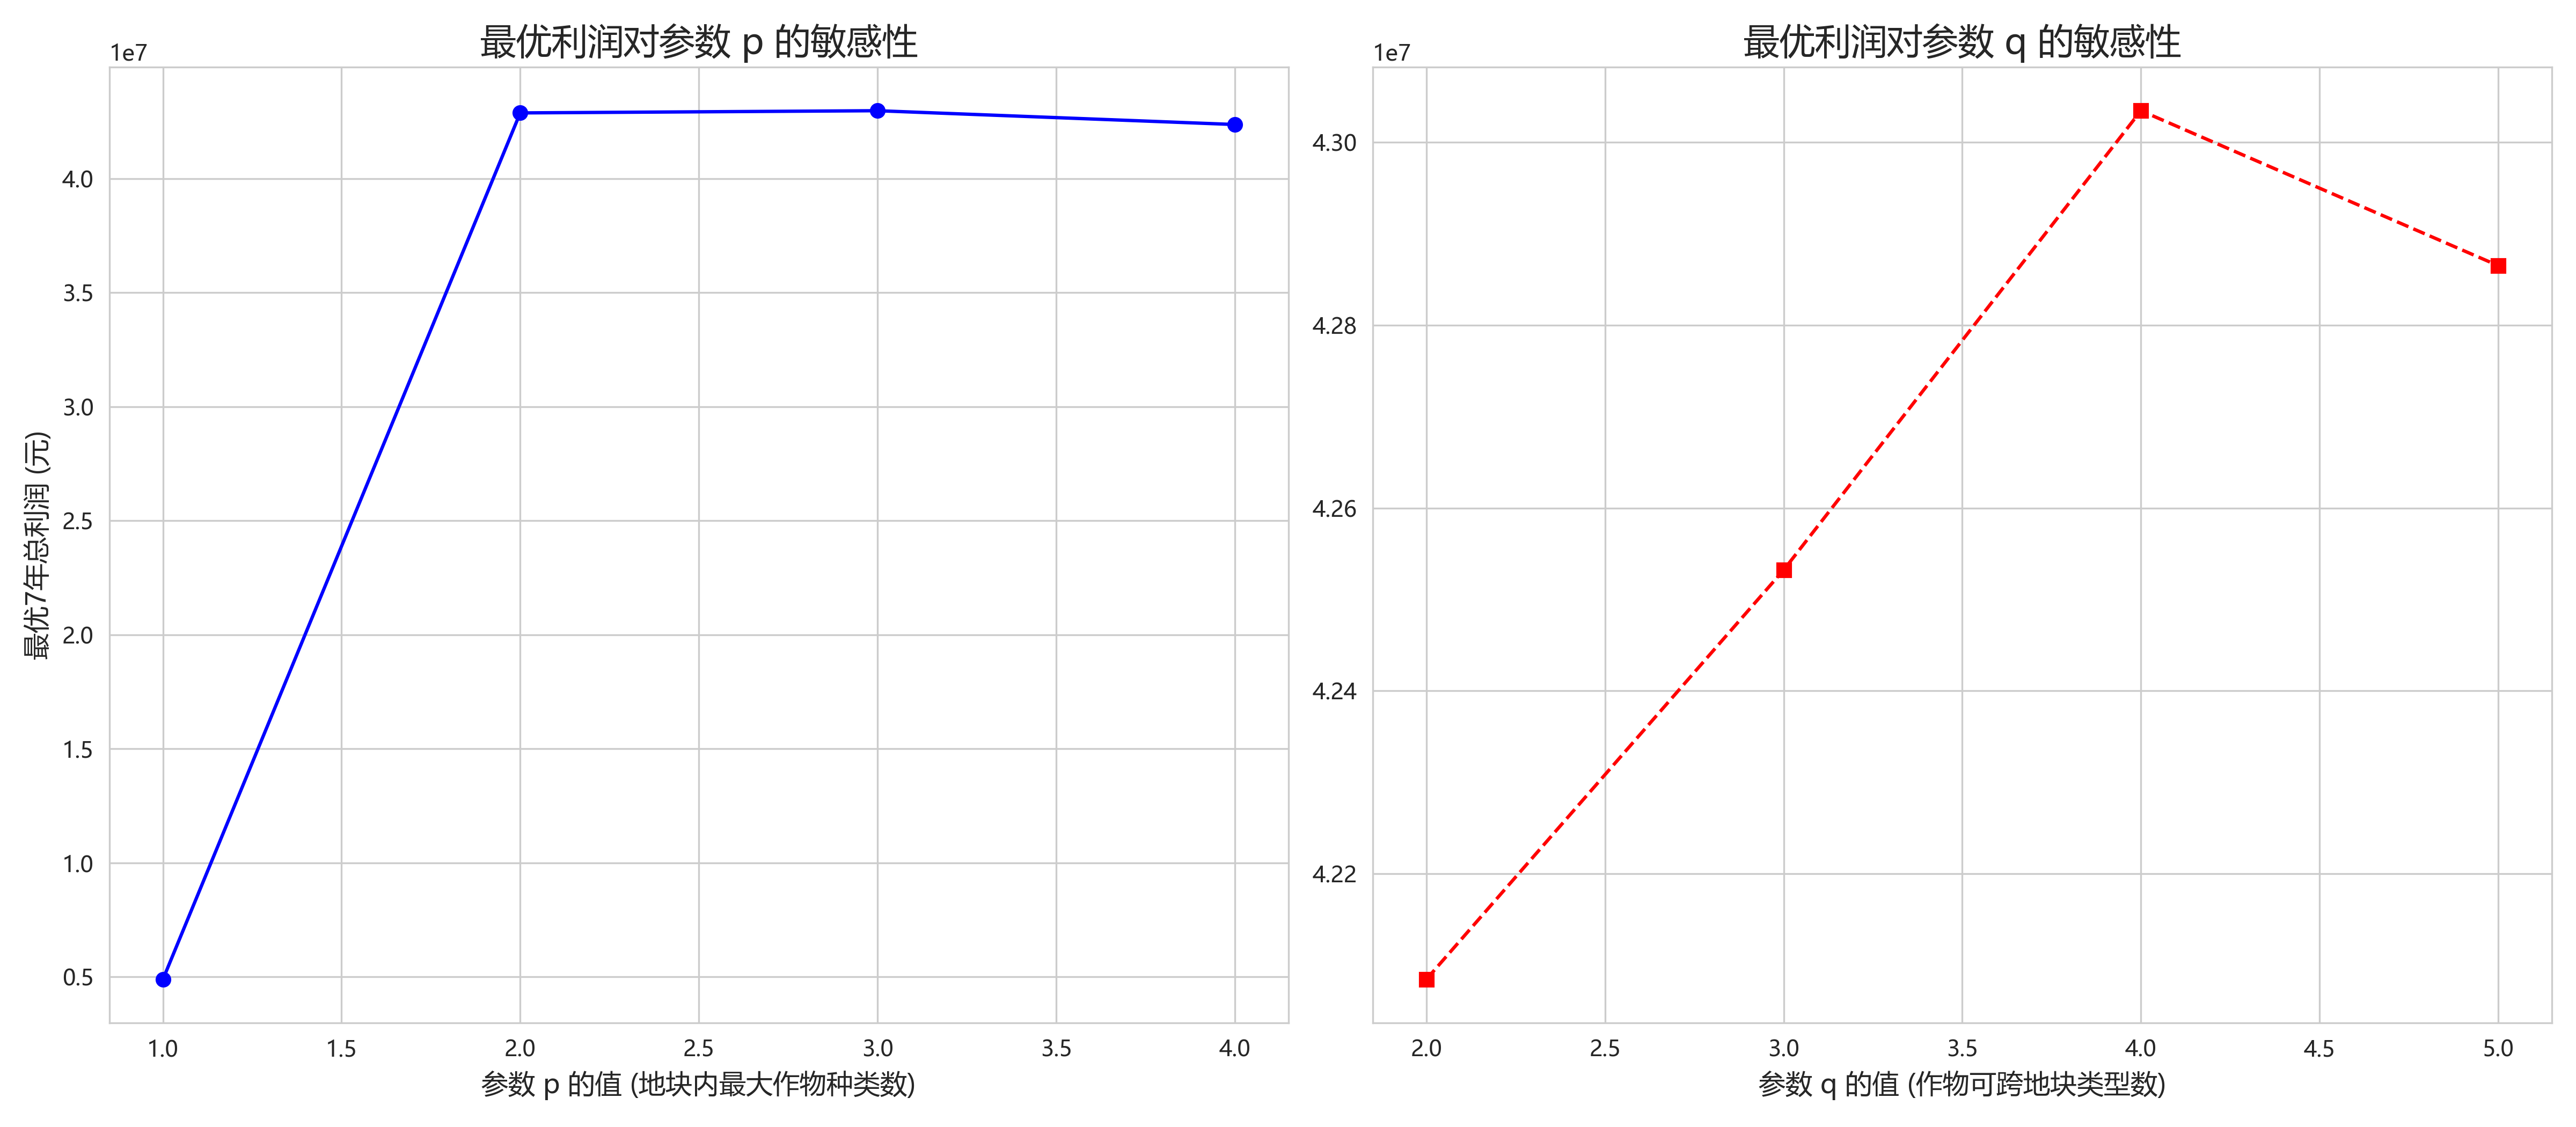
\includegraphics[width=0.9\textwidth]{figs/3问题一/pq灵敏度分析.png}
    \caption{总利润对管理便利性参数 $p$ (左) 和 $q$ (右) 的灵敏度分析。}
    \label{fig:pq_sensitivity}
\end{figure}

\subsubsection{关键土地资源面积的灵敏度分析}

土地是农业生产最基础的资源,不同类型土地的经济价值存在显著差异。为了识别对总体经济效益影响最大的土地类型,我们选取了智慧大棚、普通大棚和水浇地这三类高价值土地,对其总面积进行$\pm20\%$范围内的缩放,分析总利润的相应变化。

如图\ref{fig:area_sensitivity}所示,基准方案(所有土地面积为100\%)的七年总利润为3930万元。分析结果清晰地表明,总利润对智慧大棚面积的变化最为敏感。其对应的曲线(绿色)斜率最大,当智慧大棚面积从基准增加20\%时,总利润能提升至近4400万元;反之,若减少20\%,利润则会降至约3700万元。相比之下,普通大棚(蓝色曲线)和水浇地(青色曲线)面积变化对总利润的影响则温和得多。

这一发现具有明确的经济学意义:智慧大棚是该乡村最为关键和高效的生产资产。因此,从资源配置和未来投资的角度看,任何旨在增加智慧大棚面积的举措,都将是提升该乡村农业经济效益的最有效途径。

\begin{figure}[H]
    \centering
    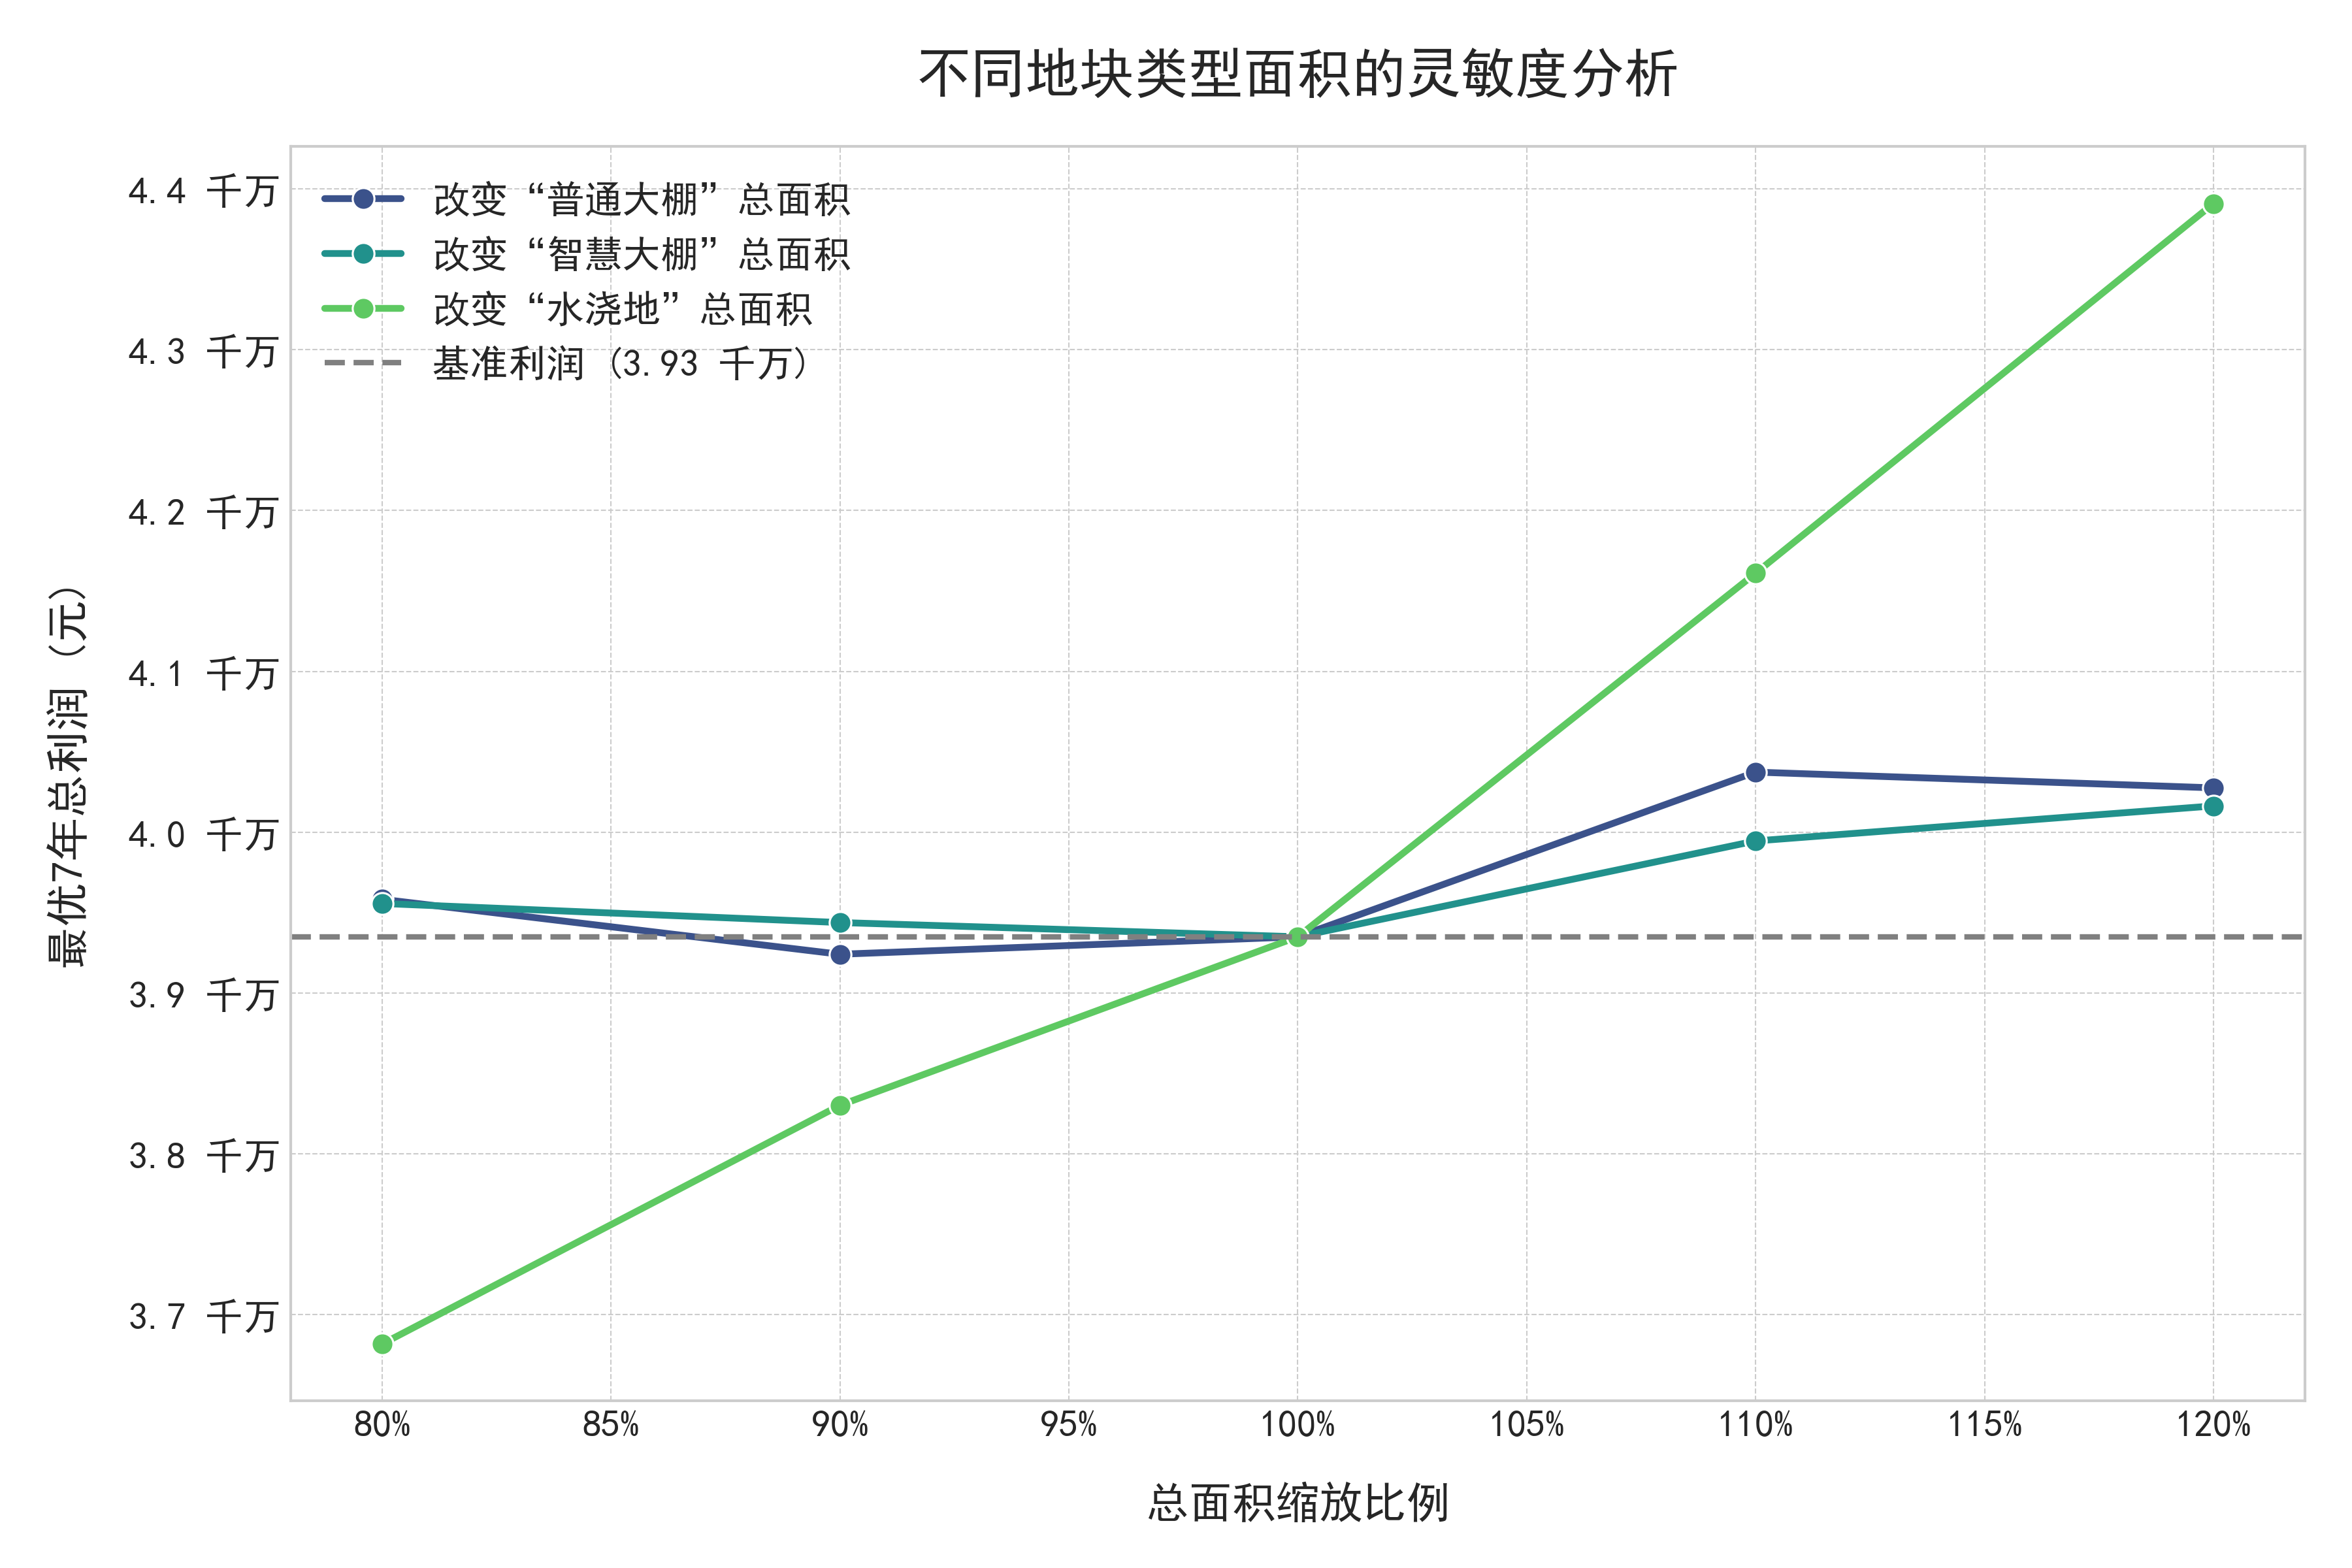
\includegraphics[width=0.8\textwidth]{figs/3问题一/面积灵敏度分析.png}
    \caption{总利润对关键土地资源总面积的灵敏度分析。}
    \label{fig:area_sensitivity}
\end{figure}


\section{问题二:不确定性环境下的鲁棒优化模型}

面对未来市场与生产环境中的不确定性,原有的确定性优化模型已不再适用。问题二的核心要求,是从寻求单一情景下的最优解,转变为在众多可能的未来情景中,制定一个能够抵御风险、综合表现稳健的种植策略。为此,本章建立了一个鲁棒优化框架,如图\ref{fig:robustness_framework}所示。该框架的目标是在所有预设的不确定性扰动下,寻求一个能够保障最低利润水平的种植方案。


\begin{figure}[H]
	\centering
	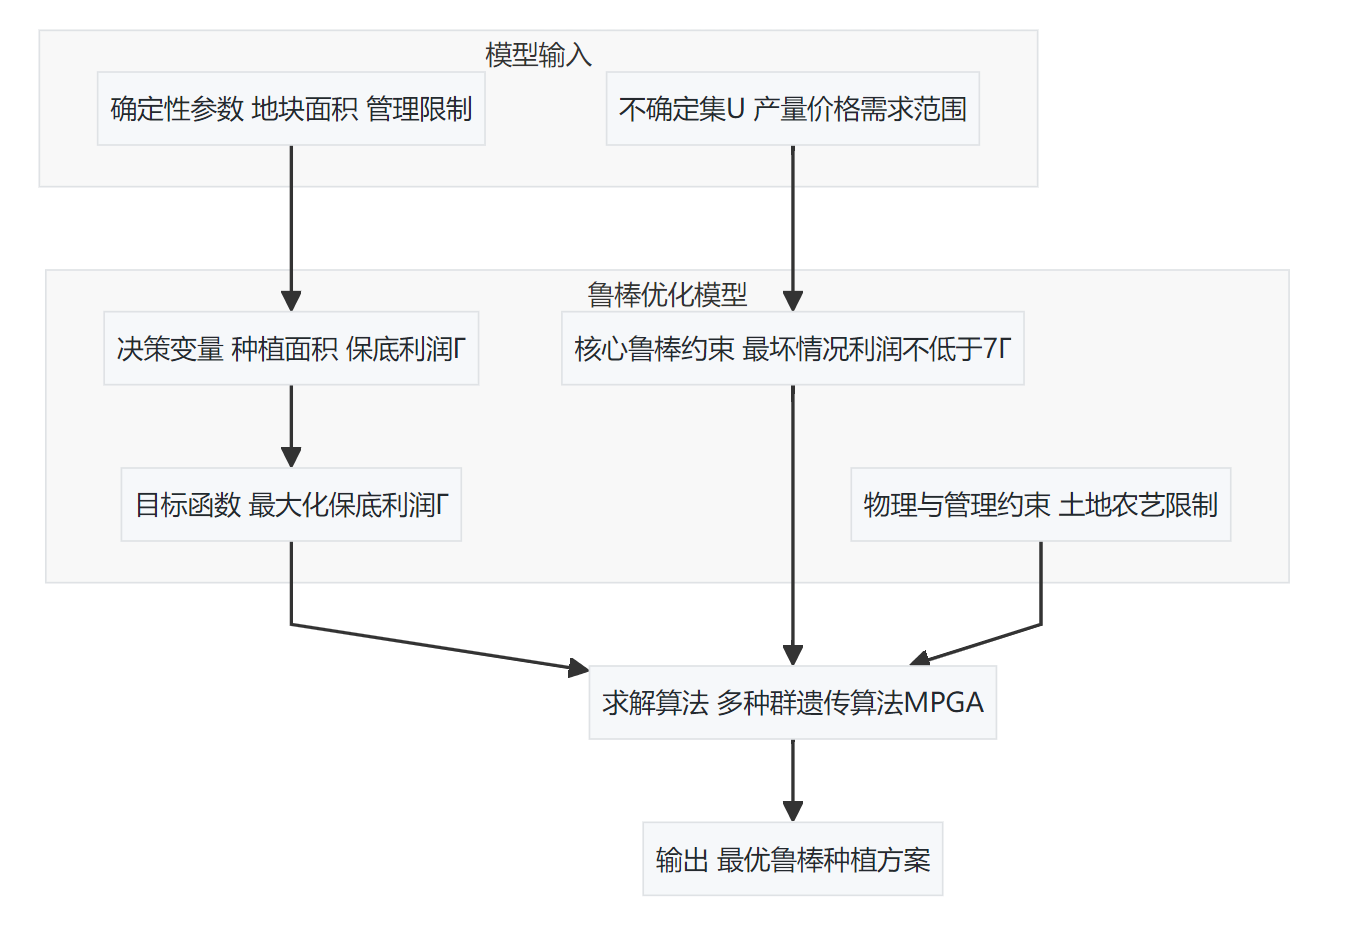
\includegraphics[width=0.9\textwidth]{figs/4问题二/问题二框架.png}
	\caption{鲁棒优化框架}
	\label{fig:robustness_framework}
\end{figure}


\subsection{模型构建}
我们选择以问题一中的情景二作为市场基础反应机制,即产量超出预期的部分按正常价格的50\%销售。我们认为这种设定比完全滞销更能反映现实市场的供需调节能力,并在此基础上构建鲁棒优化模型\upcite{YCGL202408011}。

\vspace{1cm}

\subsubsection{参数与不确定集}
模型参数分为确定性与不确定性两类。地块面积 $A_i$、地块内作物种类上限 $p$、作物跨地块类型上限 $q$ 等属于确定性参数。另一部分关键参数则是不确定的,它们在一个预设的区间(即不确定集 $U$)内波动。
\begin{itemize}
	\item \textbf{亩产量 ($yield_{jy}$)}: 受气候等因素影响,年亩产量在上一年度基准值的90\%至110\%之间波动。
	\item \textbf{预期销售量 ($sale_{jy}$)}: 小麦和玉米的需求呈增长趋势,年增长率介于5\%至10\%;其他作物的年需求量则在上一年度基准值的95\%至105\%之间变动。
	\item \textbf{种植成本 ($C_{jy}$)}: 成本被视为确定性增长,每年递增5\%。
	\item \textbf{销售价格 ($P_{jy}$)}: 粮食类价格稳定;蔬菜类价格每年增长5\%;羊肚菌价格每年下降5\%;其他食用菌价格年下降率介于1\%至5\%之间。
\end{itemize}

\vspace{1cm}

\subsubsection{决策变量与目标函数}
本模型的核心决策变量是在年份 $y$ 的第 $k$ 季,于地块 $i$ 上种植作物 $j$ 的面积 $a_{ijky}$,以及相应的二进制变量 $x_{ijky}$。此外,引入辅助变量 $normal_{jy}$ 和 $over_{jy}$ 分别表示正常销售和降价销售的产量。

区别于传统优化模型,本模型引入了一个关键的决策变量 $\Gamma$,它代表七年规划期内的年度平均保底利润。整个优化模型的目标,是最大化这个在最坏情况下依然能够实现的年度平均保底利润 $\Gamma$。
\begin{equation}
	\text{Maximize} \quad \Gamma \label{eq:objective}
\end{equation}

\vspace{1cm}

\subsubsection{约束条件}
为实现上述目标,模型建立在一系列约束之上,其中核心是鲁棒约束。
\begin{enumerate}
	\item \textbf{核心鲁棒约束}: 该约束是鲁棒优化的关键。它要求在不确定集 $U$ 内的任何一种场景组合下,七年的累计总利润都不得低于由保底利润 $\Gamma$ 定义的总目标值。
	      \begin{equation}
		      \sum_{y \in Y} \text{Profit}_y \ge 7 \cdot \Gamma, \quad \forall (yield, sale, C, P) \in U \label{eq:robust_core}
	      \end{equation}
	      其中,年度利润 $\text{Profit}_y$ 的计算方式为:
	      \begin{equation}
		      \text{Profit}_y = \sum_{j \in J} (normal_{jy} \cdot P_{jy} + over_{jy} \cdot 0.5 \cdot P_{jy}) - \sum_{i,j,k} a_{ijky} \cdot C_{jy} \label{eq:profit_calc}
	      \end{equation}

	\item \textbf{产量与销售关联约束}: 作物的总产量等于正常销售量与降价销售量之和,此关系在所有可能的亩产量场景下均须成立。
	      \begin{equation}
		      \sum_{i,k} a_{ijky} \cdot yield_{jy} = normal_{jy} + over_{jy}, \quad \forall j, y, \forall yield_{jy} \in U_{yield} \label{eq:yield_balance}
	      \end{equation}

	\item \textbf{鲁棒化的正常销售上限约束}: 为确保方案的可行性,正常价格销售的产量部分不应超过在任何需求波动下都能实现的最低预期销售量。
	      \begin{equation}
		      normal_{jy} \le \underline{sale}_{jy}, \quad \forall j,y \label{eq:sale_limit_robust}
	      \end{equation}
	      其中 $\underline{sale}_{jy}$ 是作物 $j$ 在年份 $y$ 的预期销售量下限。

	\item \textbf{物理与管理约束}: 此部分约束与问题一基本一致,包括决策变量关联、土地适宜性、地块面积限制、重茬约束、豆类轮作要求 以及作物分散性限制。
\end{enumerate}

\subsection{模型求解:多种群遗传算法}
为求解上述随机优化问题,我们采用了多种群遗传算法(Multi-Population Genetic Algorithm, MPGA)\upcite{QLJV202403012}。标准的遗传算法在处理复杂解空间时,可能因种群多样性过早丧失而收敛到局部最优解。多种群遗传算法通过将整个种群划分为若干个并行的、相对独立的子种群来应对这一挑战。每个子种群独立进行选择、交叉和变异等进化操作,这种并行搜索机制有助于维持整个种群的探索能力。具体机制如图\ref{fig:transfer_operator}所示。

\begin{figure}[H]
	\centering
	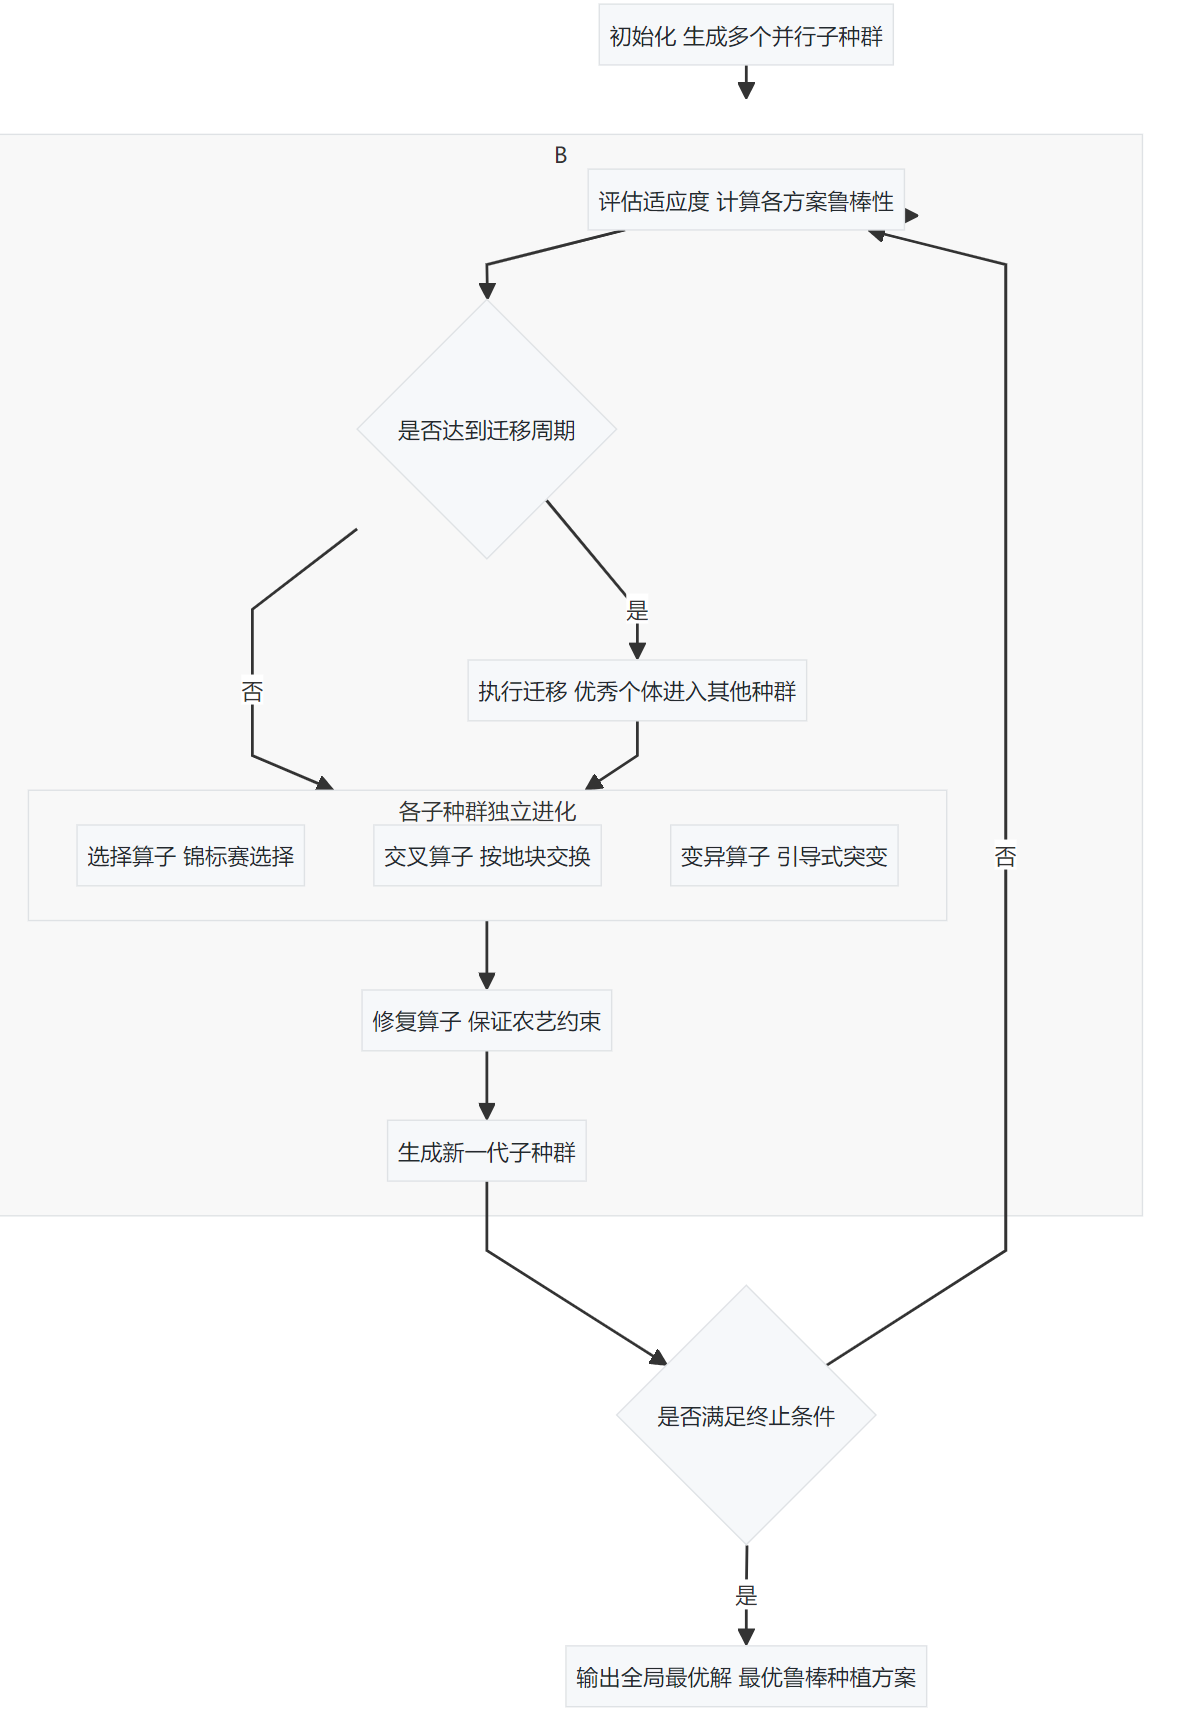
\includegraphics[width=0.8\textwidth]{figs/4问题二/多种群遗传算法.png}
	\caption{遗传算法迁移算子}
	\label{fig:transfer_operator}
\end{figure}



为促进子种群之间的信息交流,避免各个子种群陷入孤立的局部最优点,算法还引入了迁移算子。该算子以预设的代数间隔,将优势子种群中的最优个体迁移到其他子种群中,以替换其中的较差个体。这种机制使得各个子种群的优良基因得以在整个大种群中扩散,从而引导算法向全局更优的区域探索。图\ref{fig:convergence_comparison}展示了多种群遗传算法相对于标准遗传算法在收敛性能上的优势。标准算法可能在早期就陷入停滞,而多种群算法则能够持续优化,最终收敛到质量更高的解。

\begin{figure}[H]
    \centering
    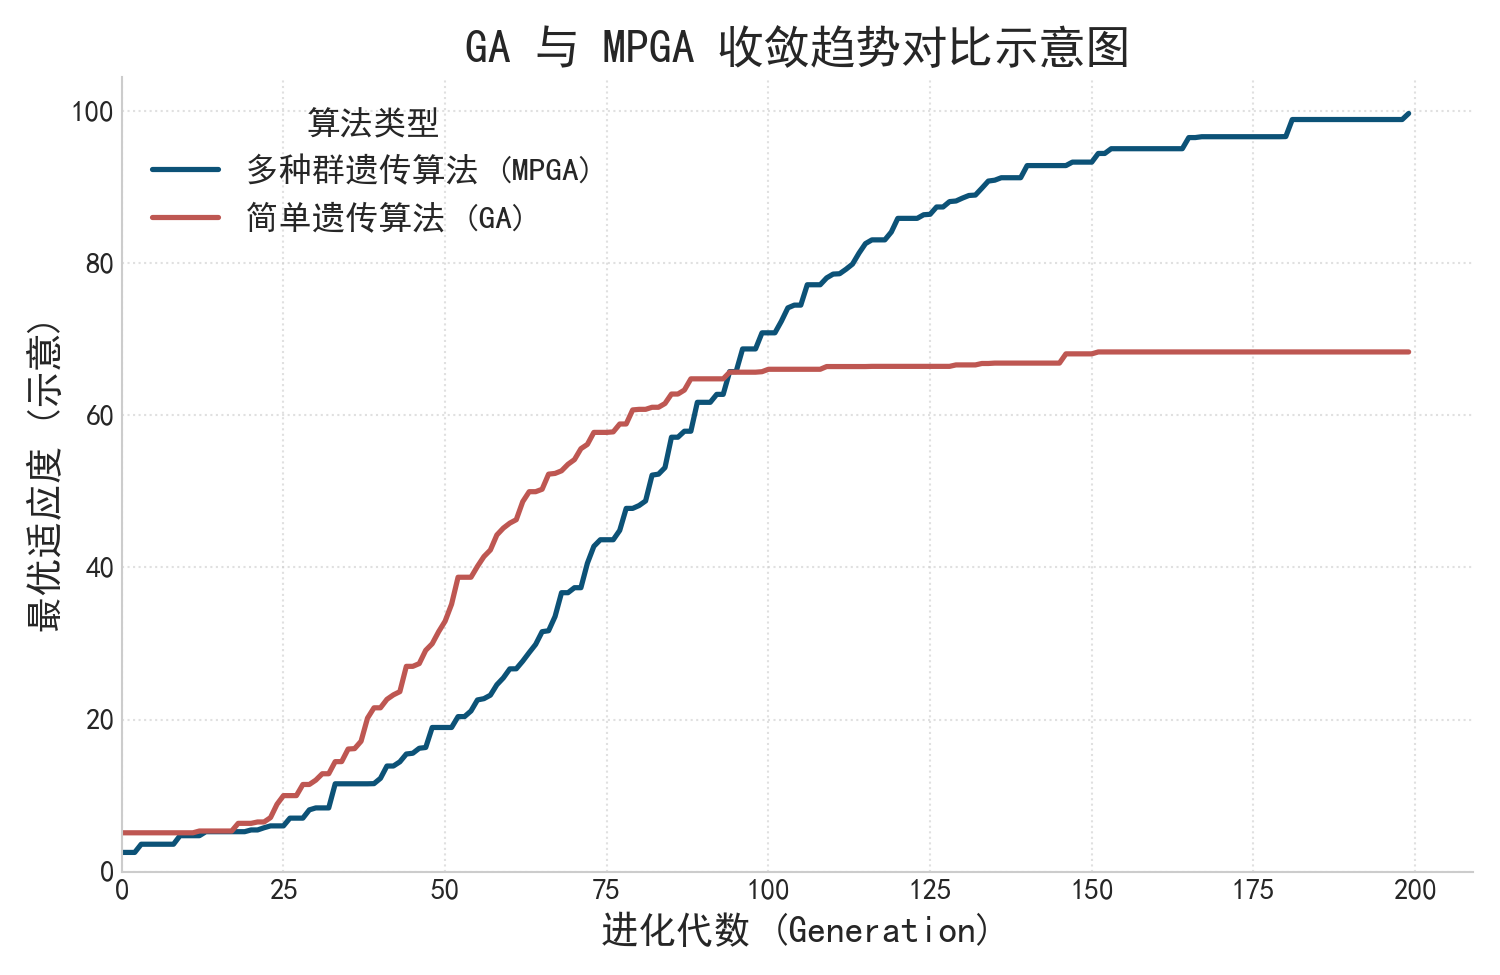
\includegraphics[width=0.7\textwidth]{figs/4问题二/遗传算法收敛对比图.png}

    \caption{多种群遗传算法与标准遗传算法收敛过程对比}
    \label{fig:convergence_comparison}
\end{figure}

算法的实现细节中,解决方案的编码、遗传算子与问题一保持一致。此外,为保证所有生成的解始终满足农艺要求,算法在每次交叉和变异操作后,均调用修复函数来处理重茬与豆类轮作这两项硬性约束。


\subsection{最优方案鲁棒性验证}


为验证本章所提出鲁棒优化方案的有效性,我们将其与问题一的情景二中得到的确定性优化方案进行了对比。两个方案在10000个相同的随机未来情景下进行模拟测试\upcite{1024787004.nh},其最终利润的统计分布如图\ref{fig:robustness_dist}所示。

\begin{figure}[H]
    \centering
    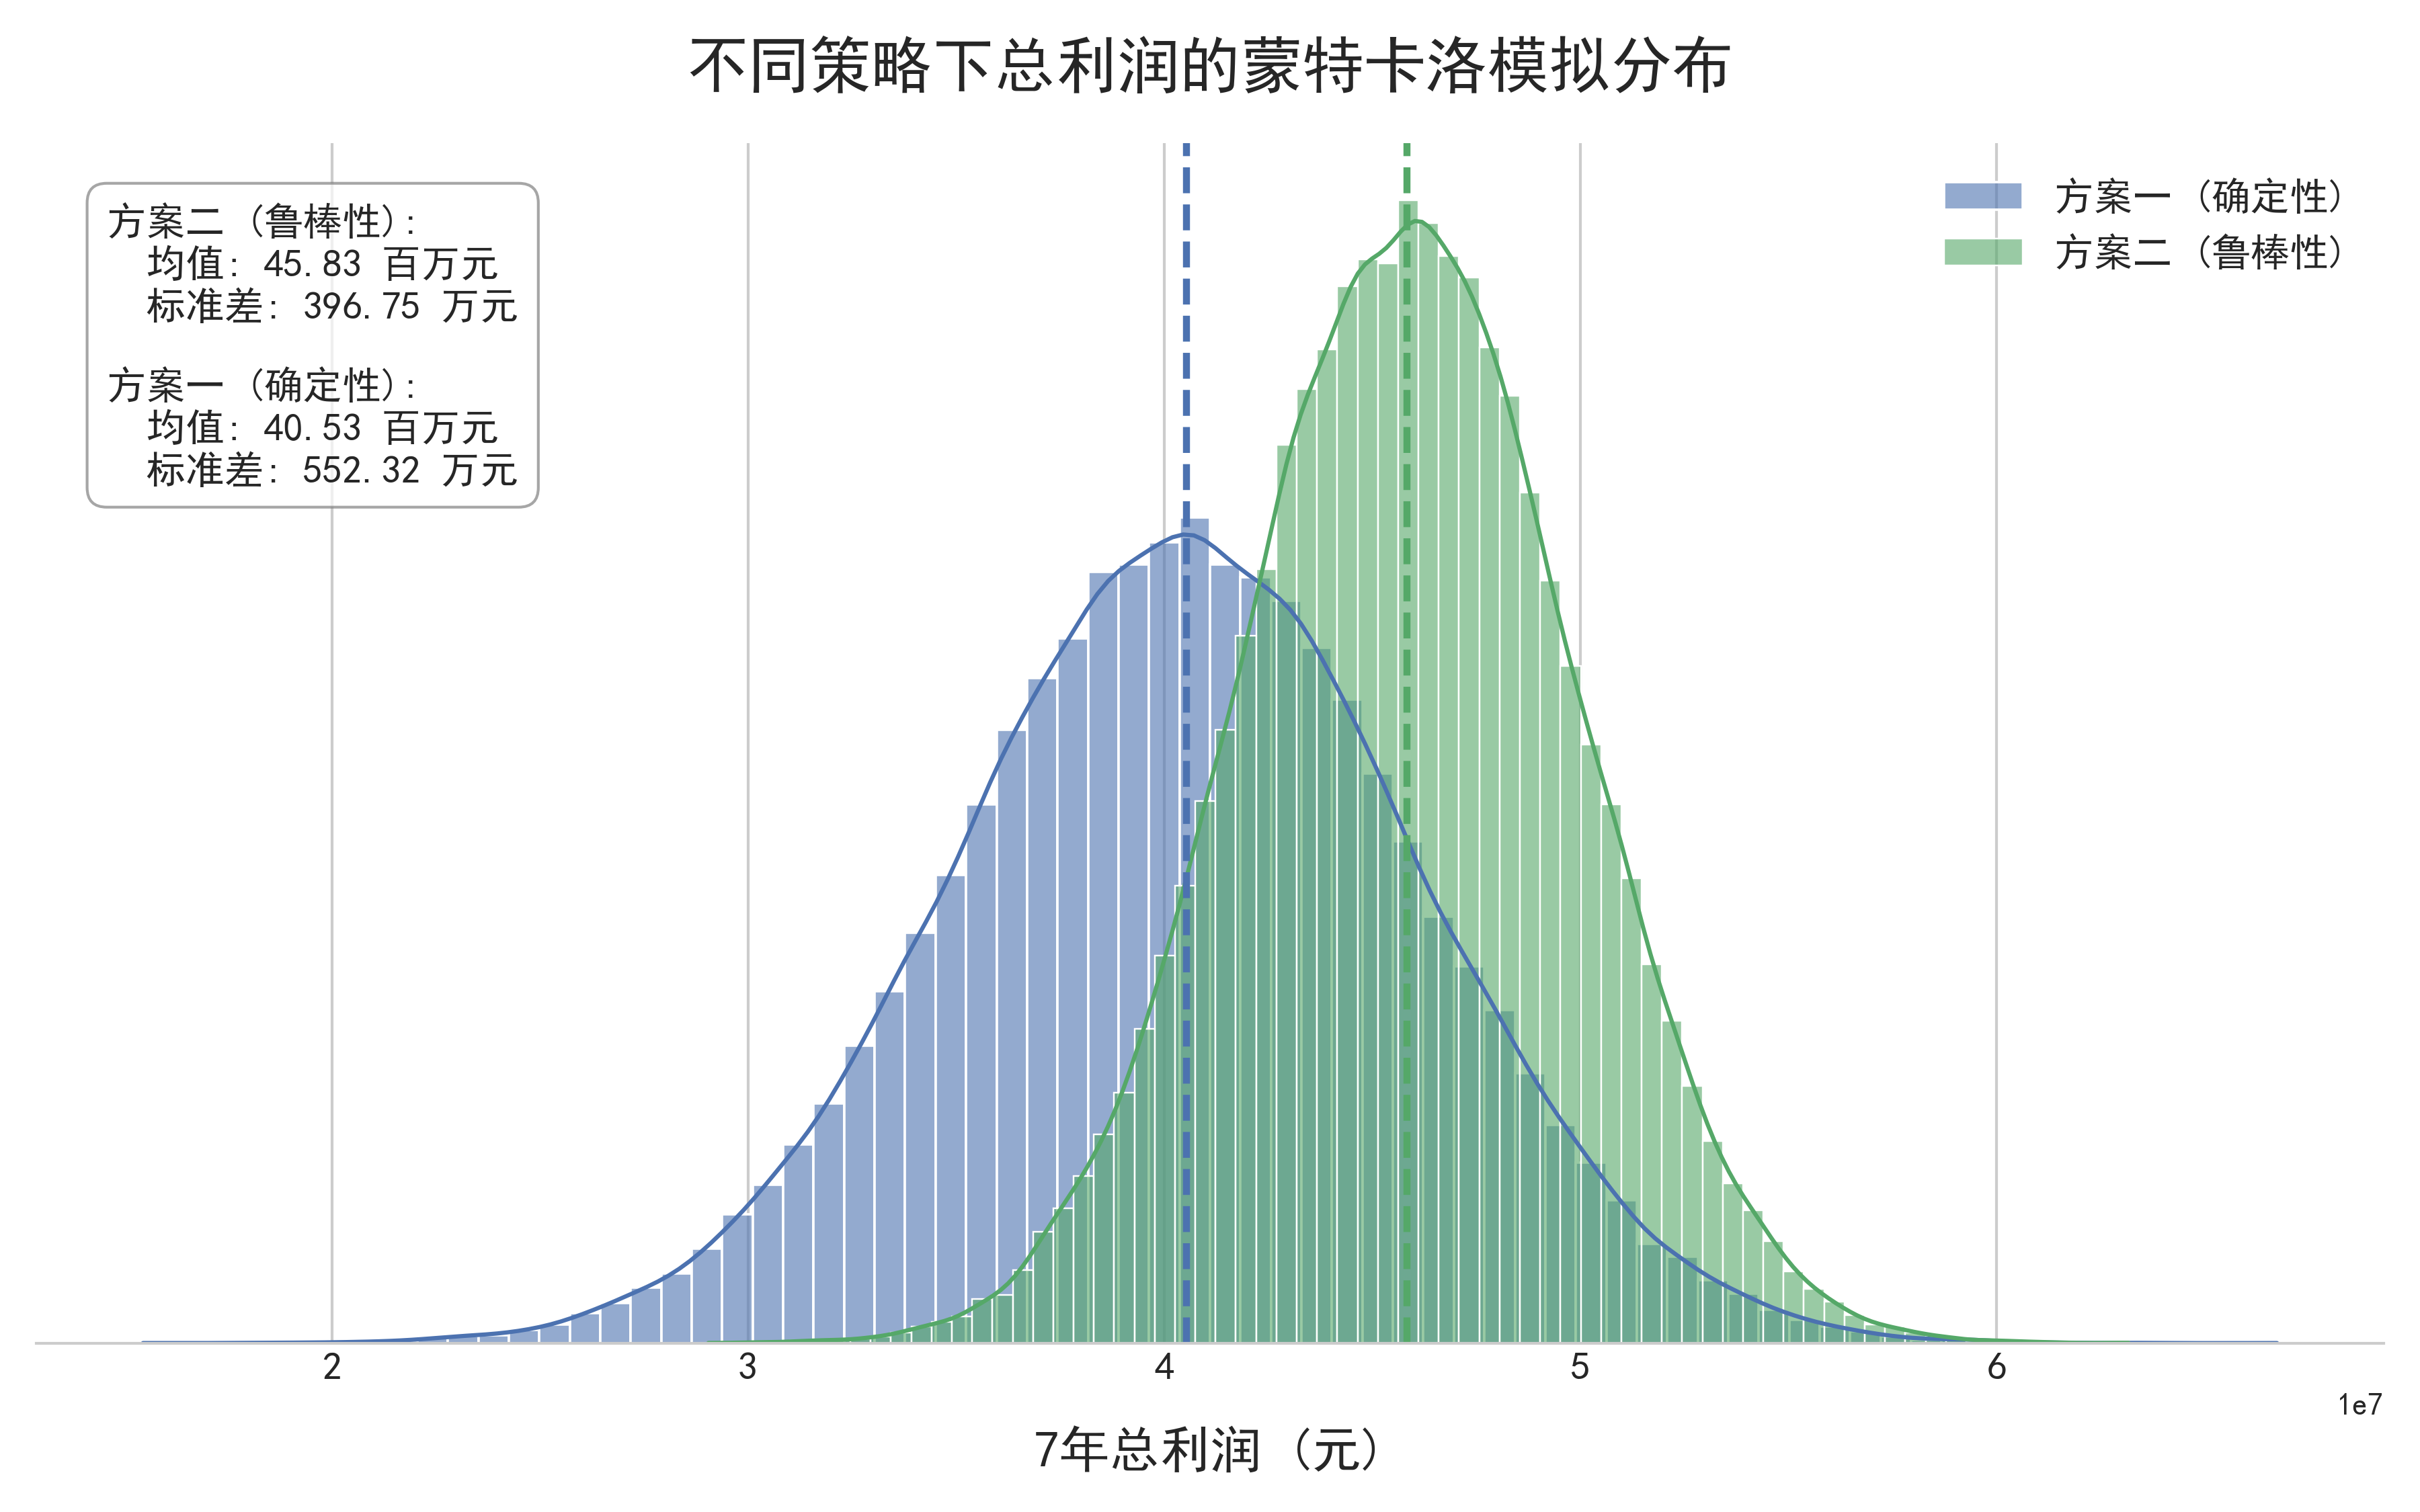
\includegraphics[width=0.8\textwidth]{figs/4问题二/鲁棒性蒙德卡诺模拟分布图.png}
    \caption{鲁棒方案与确定性方案的利润分布对比}
    \label{fig:robustness_dist}
\end{figure}

模拟结果表明,问题一的确定性方案在不确定环境下的期望利润为4.053千万元,利润标准差为0.552千万元。相比之下,本章得到的鲁棒优化方案,其期望利润提升至4.583千万元,而利润标准差则降低至0.397千万元。这一结果有力地证明,通过在优化过程中系统性地考虑不确定性,所得到的鲁棒方案不仅显著降低了未来收益的波动风险,同时也通过把握市场增长趋势,获得了更高的期望收益,其综合性能远优于确定性模型下的最优解。

\section{问题三:考虑市场动态反馈的种植策略优化}

\subsection{问题分析与建模思路}
问题二的分析是在假定市场参数的未来变化独立于乡村自身种植决策的前提下进行的。然而,在真实的经济环境中,一个区域的供给变化会对其产品的市场价格产生影响;同理,对生产资料需求的集中增加也可能推高其成本。问题三的核心即在于将这种种植决策与市场参数之间的动态反馈关系纳入模型。

为此,我们对问题二的模型框架进行拓展。基本思路是,将销售价格与种植成本的一部分变化设定为种植规模的函数。一个种植方案的总产量,将反作用于该方案在评估期内的价格与成本参数,从而影响其最终的利润表现。为实现这一目标,我们引入了量化市场反应程度的敏感度系数,并在保留原有随机波动的基础上,构建了一个更能反映市场规律的动态评估体系。由于这种反馈关系的存在,问题的求解变得更为复杂,因此我们延续并改进了在问题二中行之有效的模拟优化方法,即采用多群体遗传算法,通过大规模随机模拟来寻找在动态市场反馈下表现最优的种植方案。

\subsection{动态反馈模型的建立}

\subsubsection{市场反馈机制的数学表达}
为了将产量变化对价格和成本的影响进行数学描述,我们引入了价格敏感度系数$p_j$和成本敏感度系数$q_j$。这两个系数分别代表当作物$j$的七年平均年产量$\bar{Q_j}$相较于2023年的基准销量$S_j^{\text{base}}$超出10\%时,所引起的价格下降百分比和成本上升百分比。基于此,可定义单位超产所对应的价格调整率$\alpha_j$和成本调整率$\beta_j$:
\begin{equation}
\alpha_j = \frac{p_j}{0.1}, \quad \beta_j = \frac{q_j}{0.1}
\end{equation}
在任意一个随机情景$s$下,作物$j$的基准价格为$P_{s,j}$,基准成本为$C_{s,j}$。当种植方案确定后,其平均年产量$\bar{Q_j}$也随之确定。此时,考虑了市场反馈的调整后价格$P'_{j}$和成本$C'_{j}$由下式计算得出:
\begin{equation}
P'_{j} = P_{s,j} \cdot \left(1 - \alpha_j \cdot \max\left(0, \frac{\bar{Q_j} - 1.1 \cdot S_j^{\text{base}}}{S_j^{\text{base}}}\right)\right)
\end{equation}
\begin{equation}
C'_{j} = C_{s,j} \cdot \left(1 + \beta_j \cdot \max\left(0, \frac{\bar{Q_j} - 1.1 \cdot S_j^{\text{base}}}{S_j^{\text{base}}}\right)\right)
\end{equation}
敏感度系数的取值基于对不同作物市场特性的判断。粮食作物作为必需品,其需求价格弹性较小,因此设定其价格敏感度$p_{\text{grain}}=0.1\%$。蔬菜与食用菌的需求弹性相对更大,分别设定$p_{\text{veg}}=0.15\%$和$p_{\text{fungi}}=0.2\%$。在成本方面,粮食和蔬菜的种子、种苗市场供应体系成熟,生产要素供给弹性大,因此设定其成本敏感度$q_{\text{grain/veg}}=0.05\%$。食用菌的菌种市场相对较小,产量的大幅增加可能导致上游成本的明显上涨,故设定其成本敏感度$q_{\text{fungi}}=0.1\%$。这些参数的设定如图\ref{fig:sensitivity_setup}所示。

\begin{figure}[H]
    \centering
    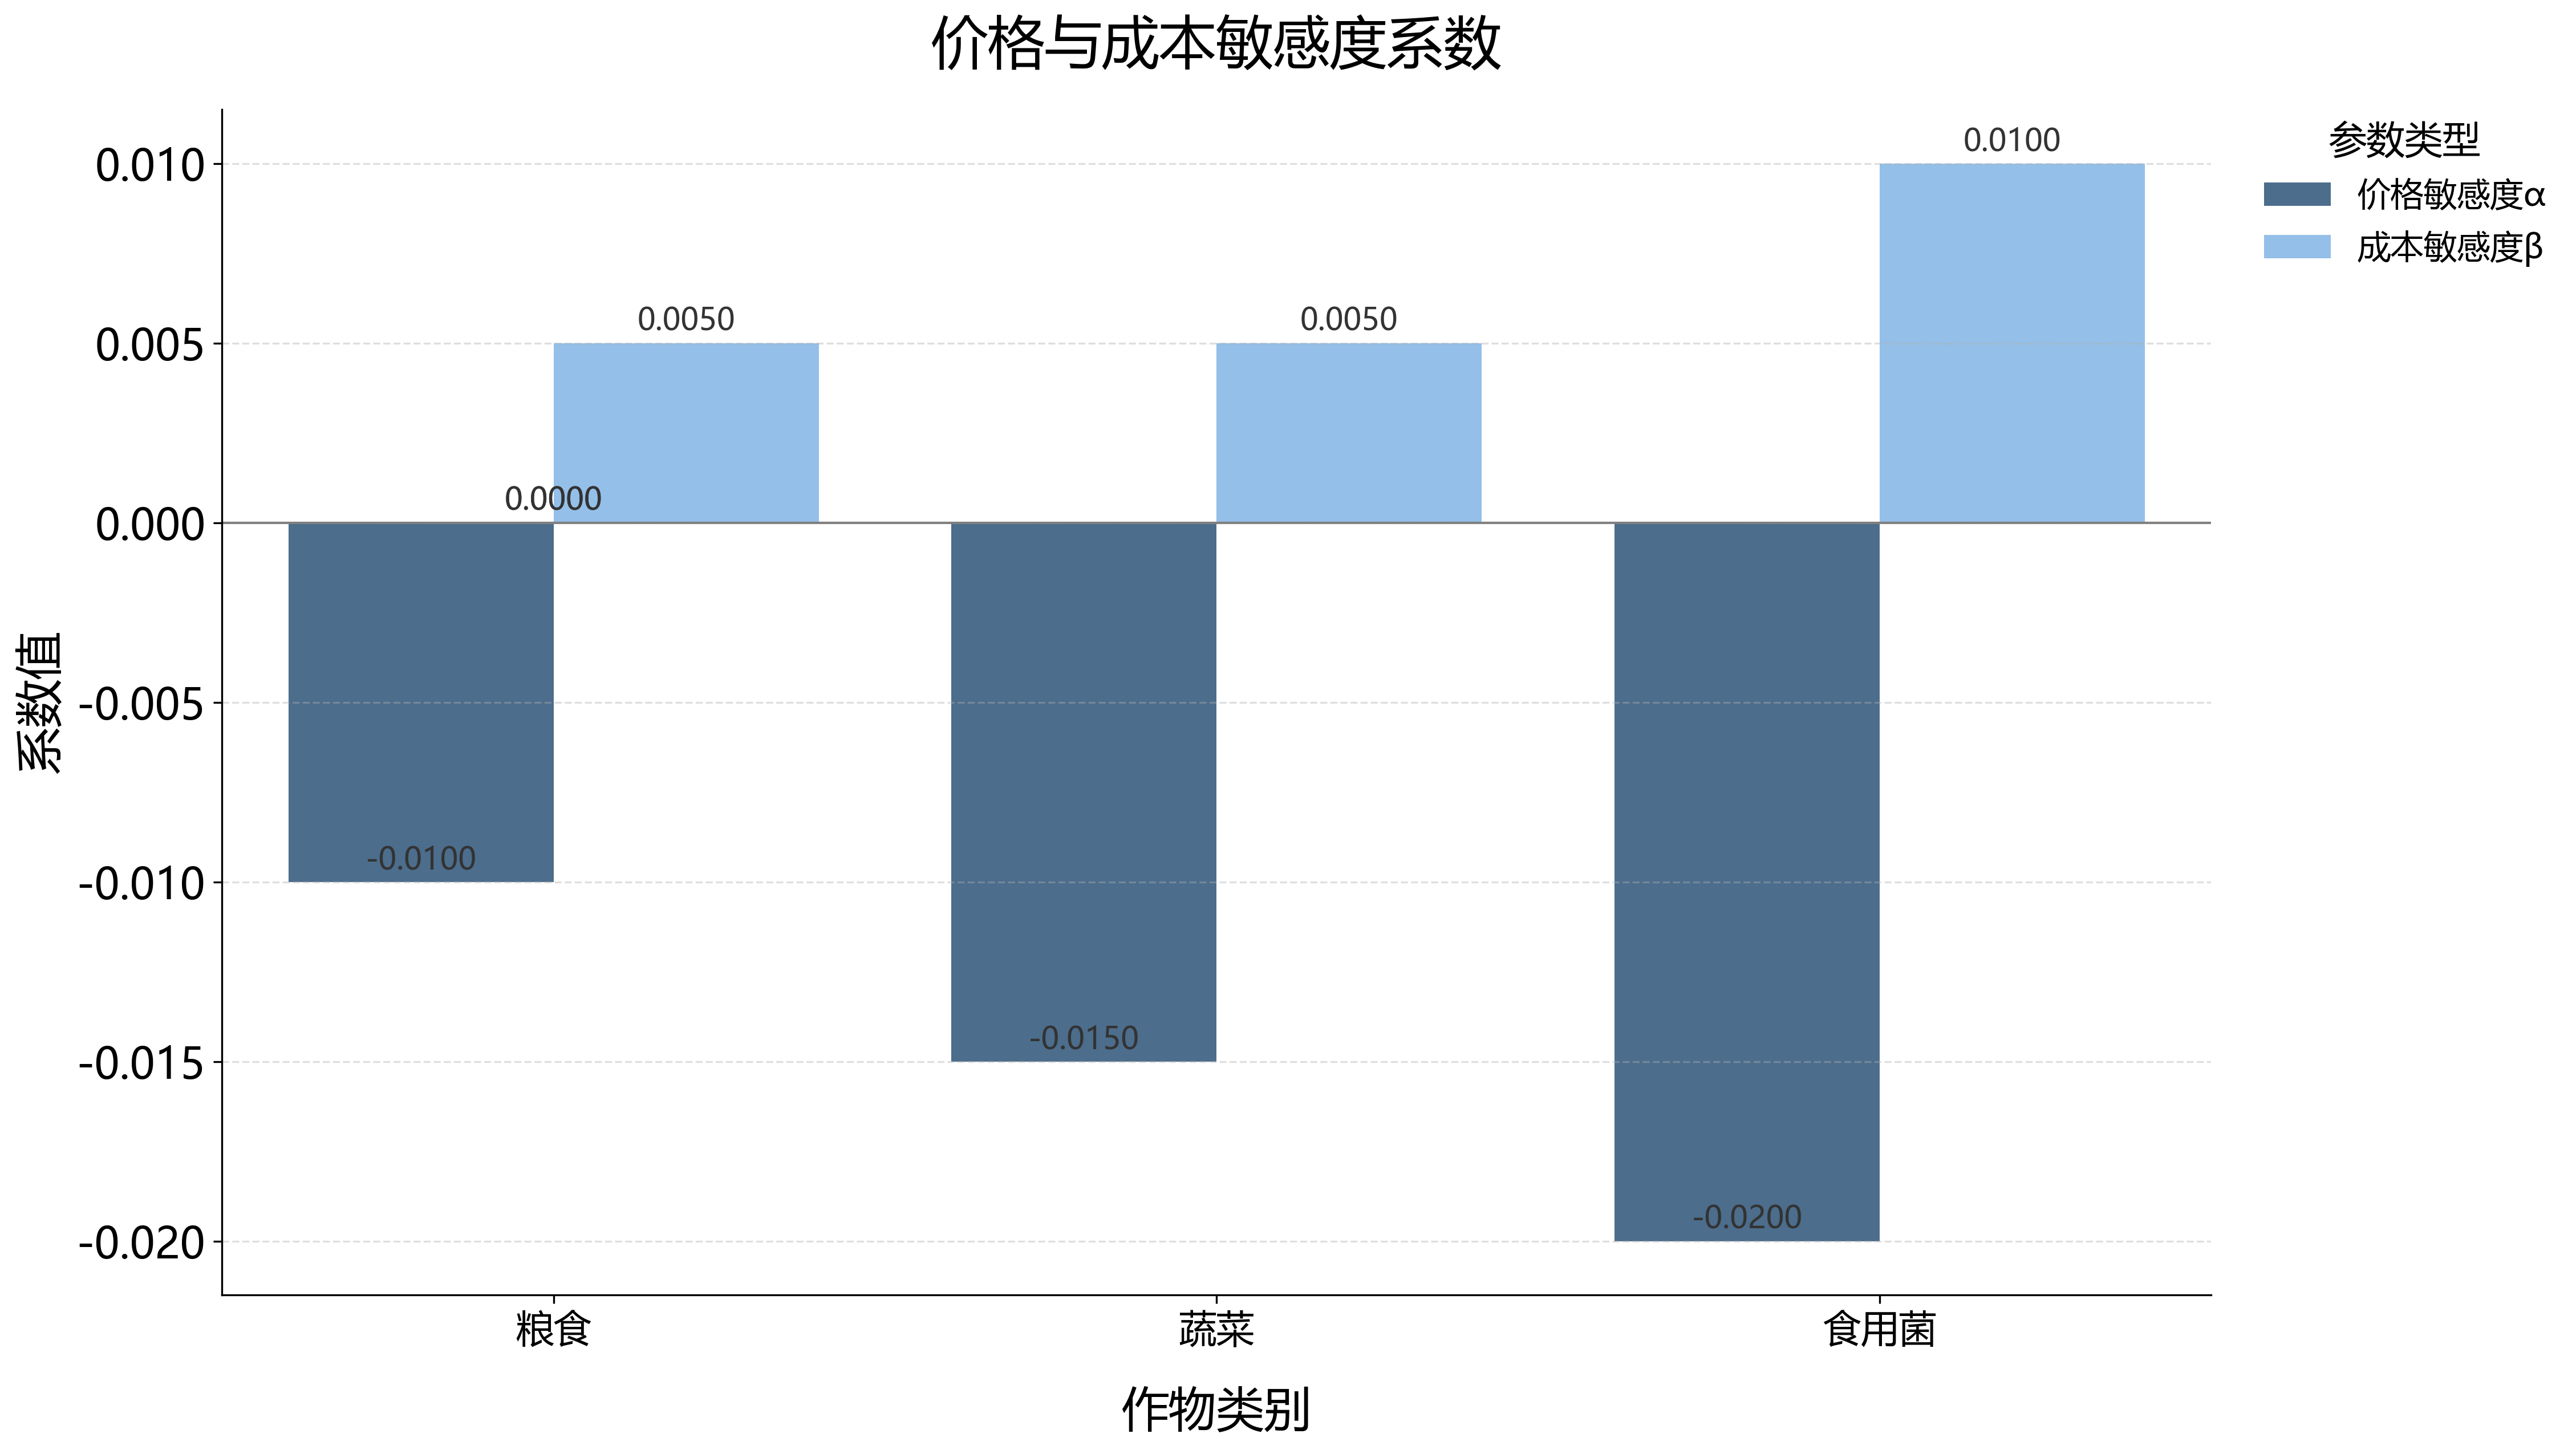
\includegraphics[width=0.9\textwidth]{figs/5问题三/敏感度系数设定图.png}
    \caption{三类作物价格与成本敏感度系数设定。}
    \label{fig:sensitivity_setup}
\end{figure}

\subsubsection{适应度函数设计}
在引入动态反馈机制后,对一个候选种植方案的优劣评估(即适应度计算)必须反映其决策对市场环境的反作用。为此,我们设计了如下的评估流程:
\begin{enumerate}
    \item 对于给定的一个七年种植方案,在其影响下,通过蒙特卡洛方法生成$N=100$组覆盖七年的随机情景。在每个情景中,计算出每种作物每年的计划产量。
    \item 基于这$N \times 7$组产量数据,计算出该方案下每种作物的七年平均年产量$\bar{Q_j}$。
    \item 使用公式(43)、(44)和(45),根据$\bar{Q_j}$计算出适用于该方案的价格与成本调整系数,并更新所有$N$个随机情景中的价格与成本数据。
    \item 基于更新后的价格与成本,重新计算该方案在所有$N$个情景下的七年总利润。
    \item 将这$N$个总利润值进行算术平均,所得结果即为该种植方案的最终适应度。
\end{enumerate}
此流程确保了适应度评价的公平性,一个试图通过过度生产某种作物以在静态市场中获利的方案,会因触发市场的负反馈机制而受到适应度惩罚。

\subsection{模型求解}
考虑到模型中包含了由产量决定的非线性动态反馈,传统的线性规划方法已不适用。因此,我们选择采用多群体遗传算法(MPGA)进行求解。该算法通过维护多个并行的子种群,并周期性地在子种群间交换优秀个体信息,有效维持了搜索过程中的种群多样性,降低了陷入局部最优解的风险,适合求解此类复杂的优化问题。算法的具体实现沿用了问题二的框架,包括采用字典结构对完整的七年种植计划进行编码,以及在遗传算子操作后调用修复函数,以确保所有候选方案始终满足禁止重茬和豆类轮作等核心农艺约束。

\subsection{求解结果与分析}

\subsubsection{最优方案的经济效益评估}
通过多群体遗传算法的迭代优化,最终得到一个综合表现最优的种植方案。为评估该方案在不确定环境下的经济效益,我们进行了100次独立的蒙特卡洛模拟。结果显示,该方案的预期七年平均总利润为\textbf{39,020,501.59元}。为进一步评估其风险水平,我们考察了利润分布的分位点。计算表明,该方案有95\%的概率实现不低于\textbf{38,651,785.03元}的总利润,同时有5\%的机会冲击\textbf{39,341,535.57元}以上的总利润。利润的5\%分位点与95\%分位点之间的区间宽度仅占期望利润的1.77\%,这表明方案的最终收益非常稳定,具有很强的抗风险能力。

\subsubsection{最优方案结构可视化分析}
为了深入理解最优方案的内在逻辑与时空布局,我们从宏观到微观,通过一系列可视化图表进行解析。

首先,图\ref{fig:optimal_solution_2024}以热力图的形式,直观展示了规划第一年(2024年)的种植安排。图中清晰地反映了不同地块的专业化分工:大棚设施(E、F类)被专门用于种植高价值的蔬菜和食用菌,水浇地(D类)则混合种植蔬菜和水稻,而大面积的平旱地、梯田和山坡地(A、B、C类)则构成了粮食作物生产的主体。

\begin{figure}[H]
    \centering
    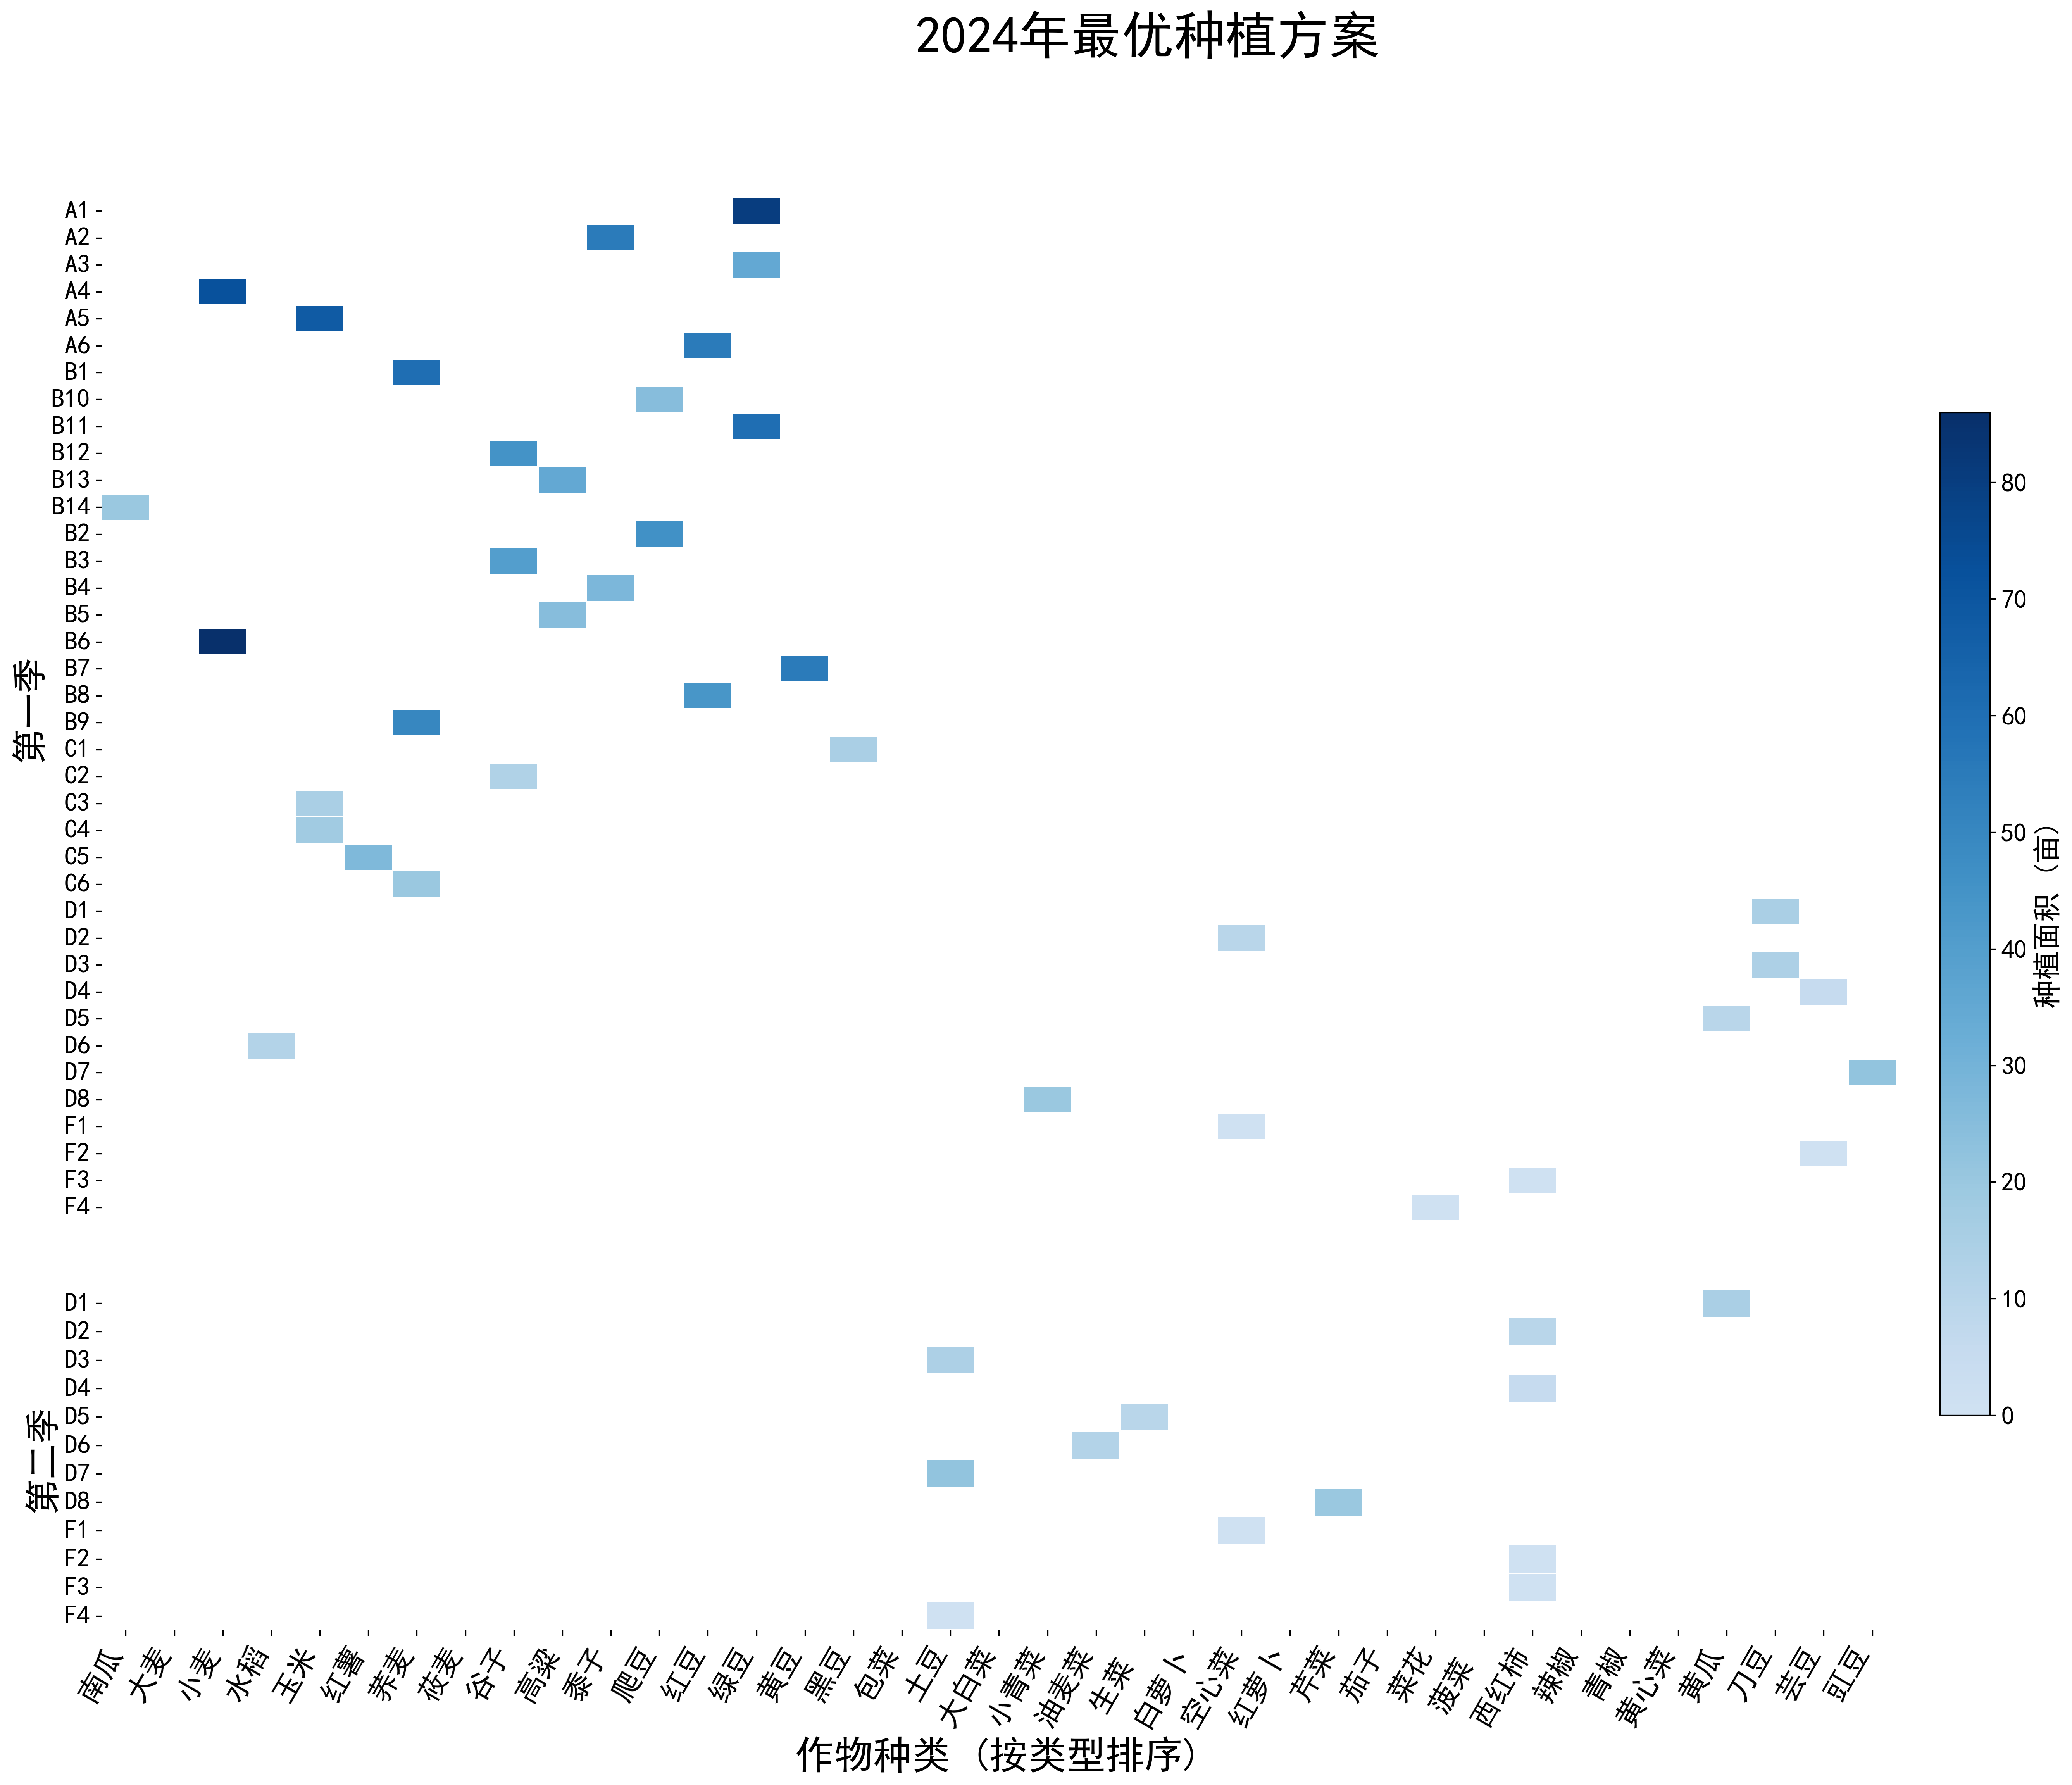
\includegraphics[width=0.7\textwidth]{figs/5问题三/2024年最优种植方案.png}
    \caption{2024年最优种植方案时空分布热力图。}
    \label{fig:optimal_solution_2024}
\end{figure}

其次,图\ref{fig:area_stack}从时间演化的角度,展示了未来七年三大类作物种植面积的年度分配。粮食作物的总面积构成了种植结构的主体,并保持相对稳定,保障了基本的粮食供给。蔬菜作物的种植面积呈现出稳步增长的态势,反映了方案在追求更高经济效益。食用菌的种植面积则保持恒定,这与大棚资源的总量限制相符。

\begin{figure}[H]
    \centering
    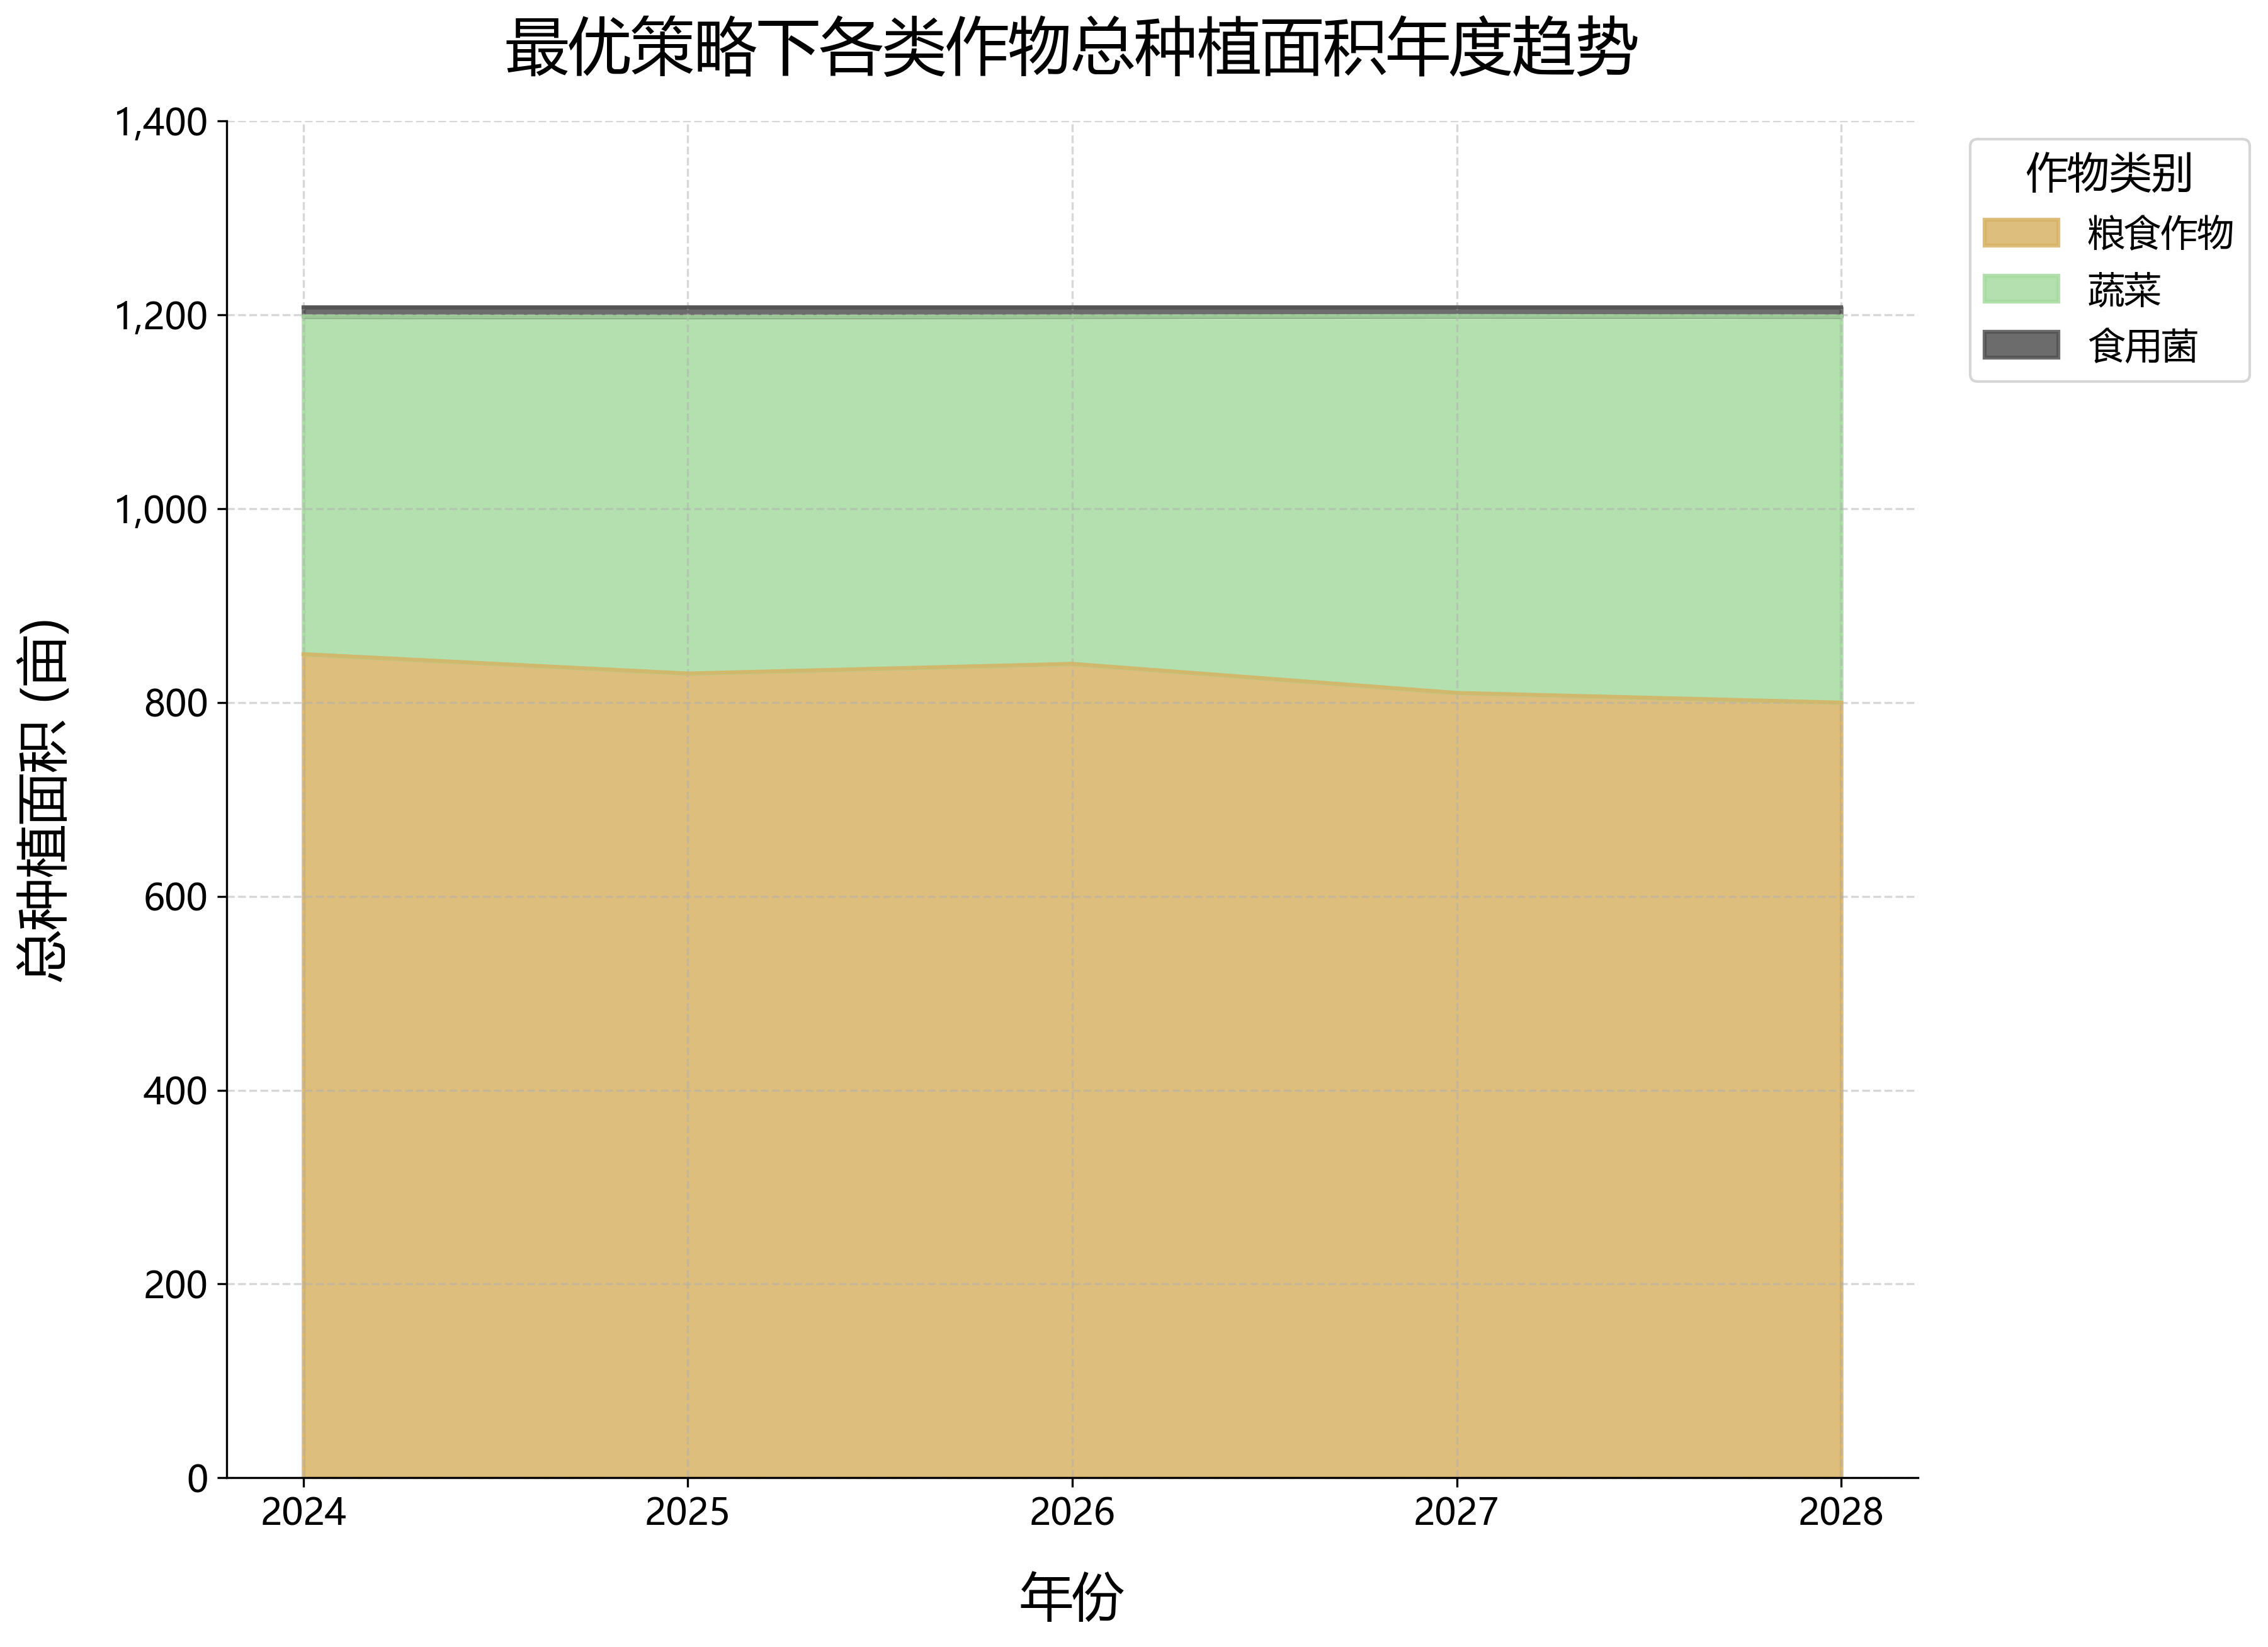
\includegraphics[width=\textwidth]{figs/5问题三/年度种植面积堆叠图_最终参考版.png}
    \caption{最优方案下2024-2030年各类作物种植面积变化趋势。}
    \label{fig:area_stack}
\end{figure}

再次,我们选取四种代表性地块,展示其详细的七年轮作计划,如图\ref{fig:plot_plan}所示。该图微观地揭示了方案的精细化程度。例如,在智慧大棚F1中,实现了蔬菜的有序轮作;在普通大棚E1中,则是一季蔬菜与一季食用菌的交替种植。平旱地A1和水浇地D1的轮作计划则清晰地展示了豆类作物被周期性地插入种植周期中,这直观地证明了方案严格遵守了“三年至少一次豆类”的农艺要求。

\begin{figure}[H]
    \centering
    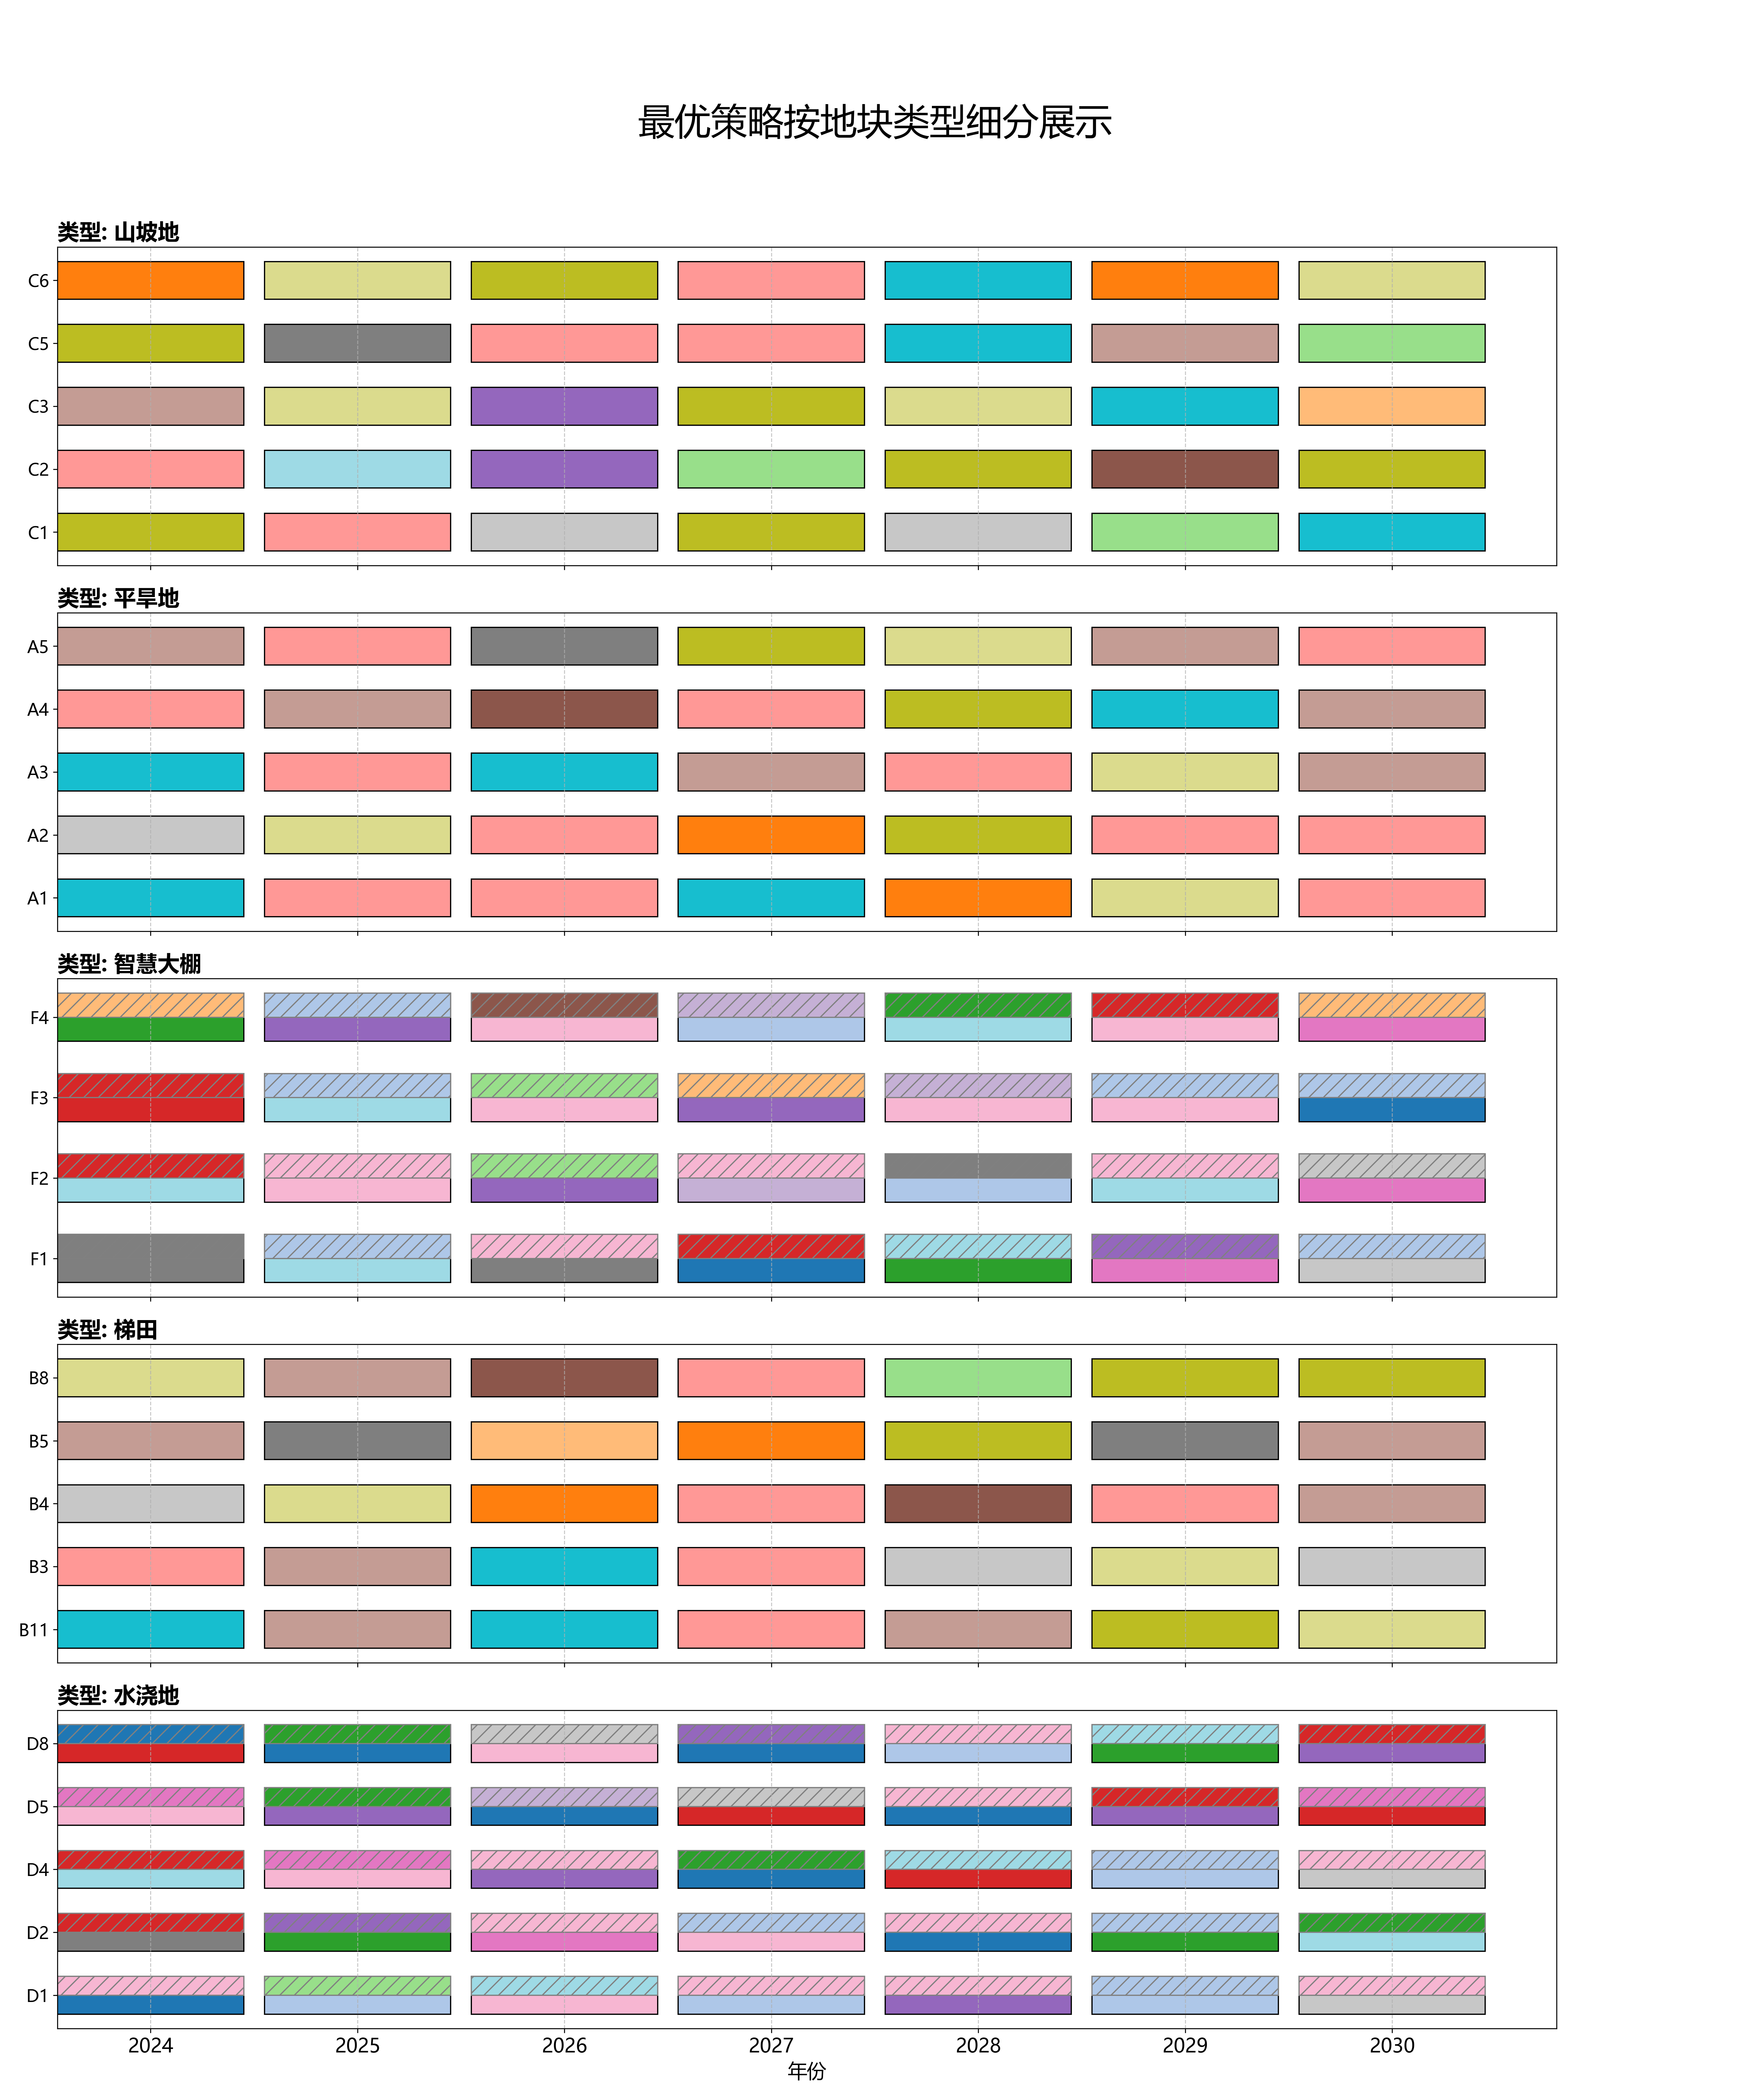
\includegraphics[width=\textwidth]{figs/5问题三/典型地块种植计划图.png}
    \caption{四类典型地块的七年详细种植计划。}
    \label{fig:plot_plan}
\end{figure}

最后,图\ref{fig:profit_dist}是本次优化成果的核心体现。该利润分布直方图展示了在考虑所有不确定性与市场反馈后,最终方案的收益并非一个确定值,而是一个紧密围绕期望值波动的概率分布。分布形态集中且偏态较小,再次印证了该方案的稳健性。

\begin{figure}[H]
    \centering
    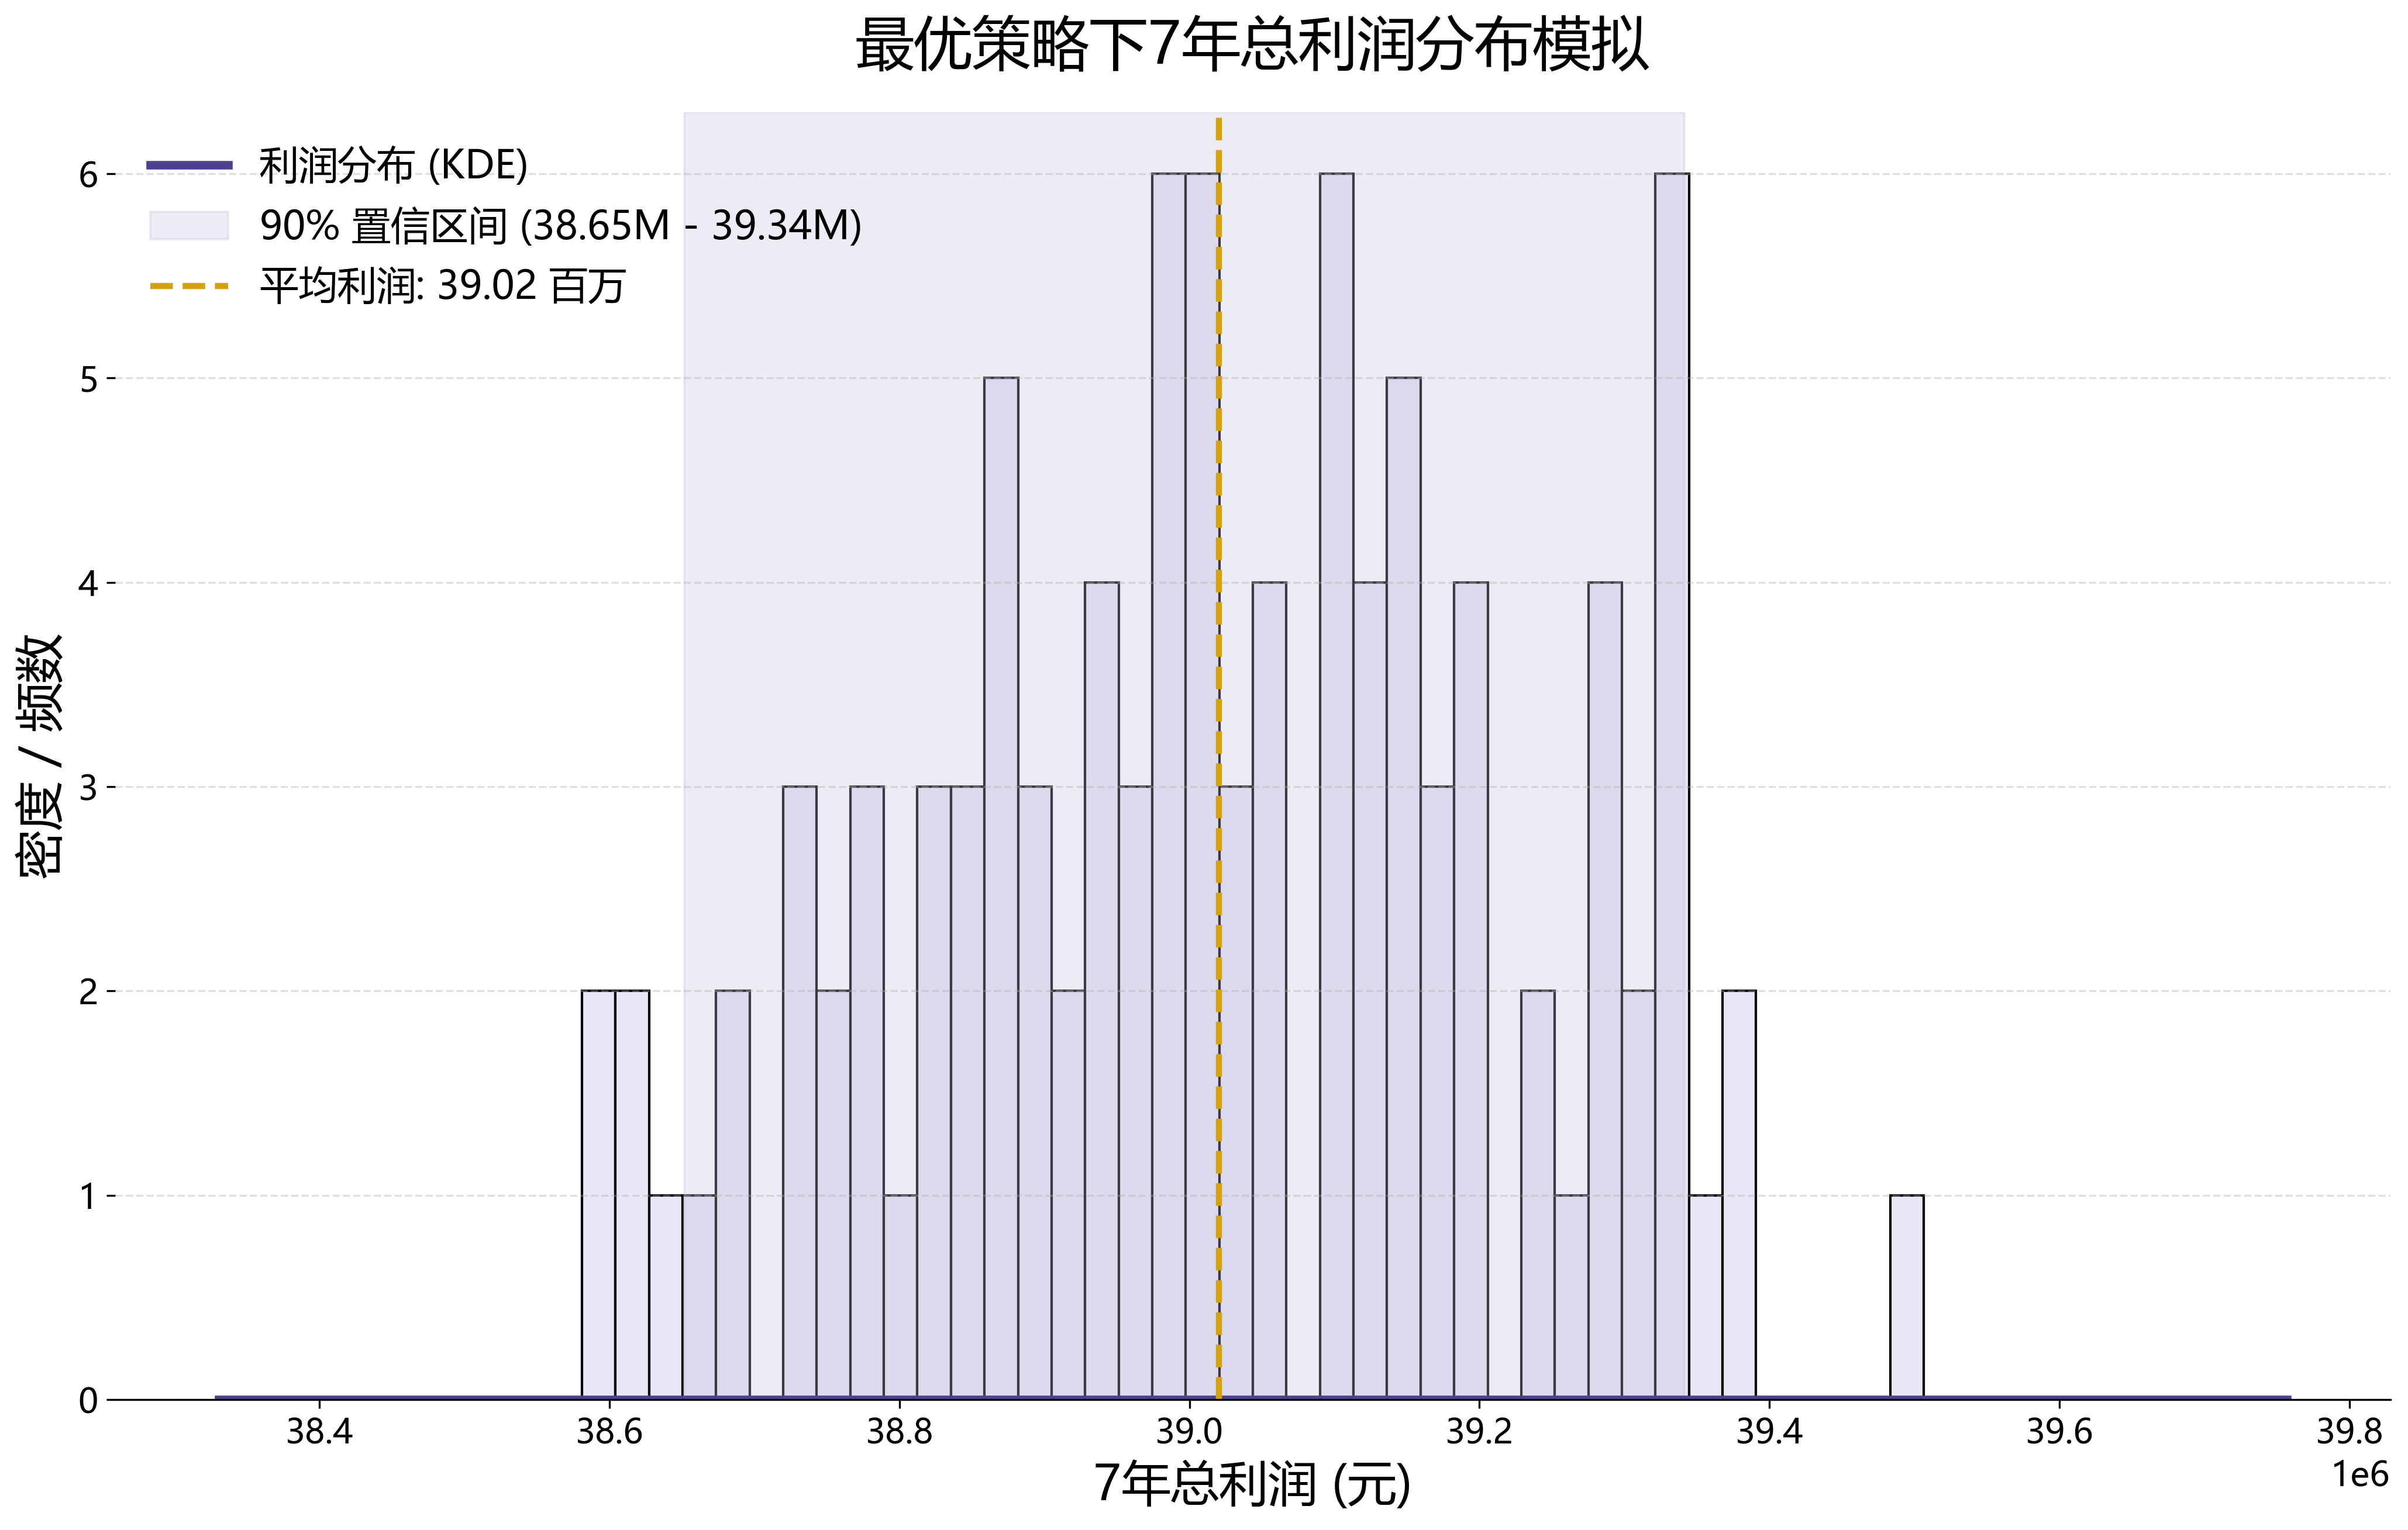
\includegraphics[width=0.9\textwidth]{figs/5问题三/利润分布图.png}
    \caption{最优方案在100次蒙特卡洛模拟下的七年总利润分布。}
    \label{fig:profit_dist}
\end{figure}

\subsection{灵敏度分析}
为检验模型结果对关键假设参数的稳健性,我们对设定的六个市场敏感度系数(三类作物的价格敏感度与成本敏感度)进行了单因素灵敏度分析。在分析中,我们每次只变动一个参数,在其基准值附近取四个不同的水平,并为每个水平重新运行完整的优化过程,记录最终的预期平均利润变化。

\begin{figure}[H]
    \centering
    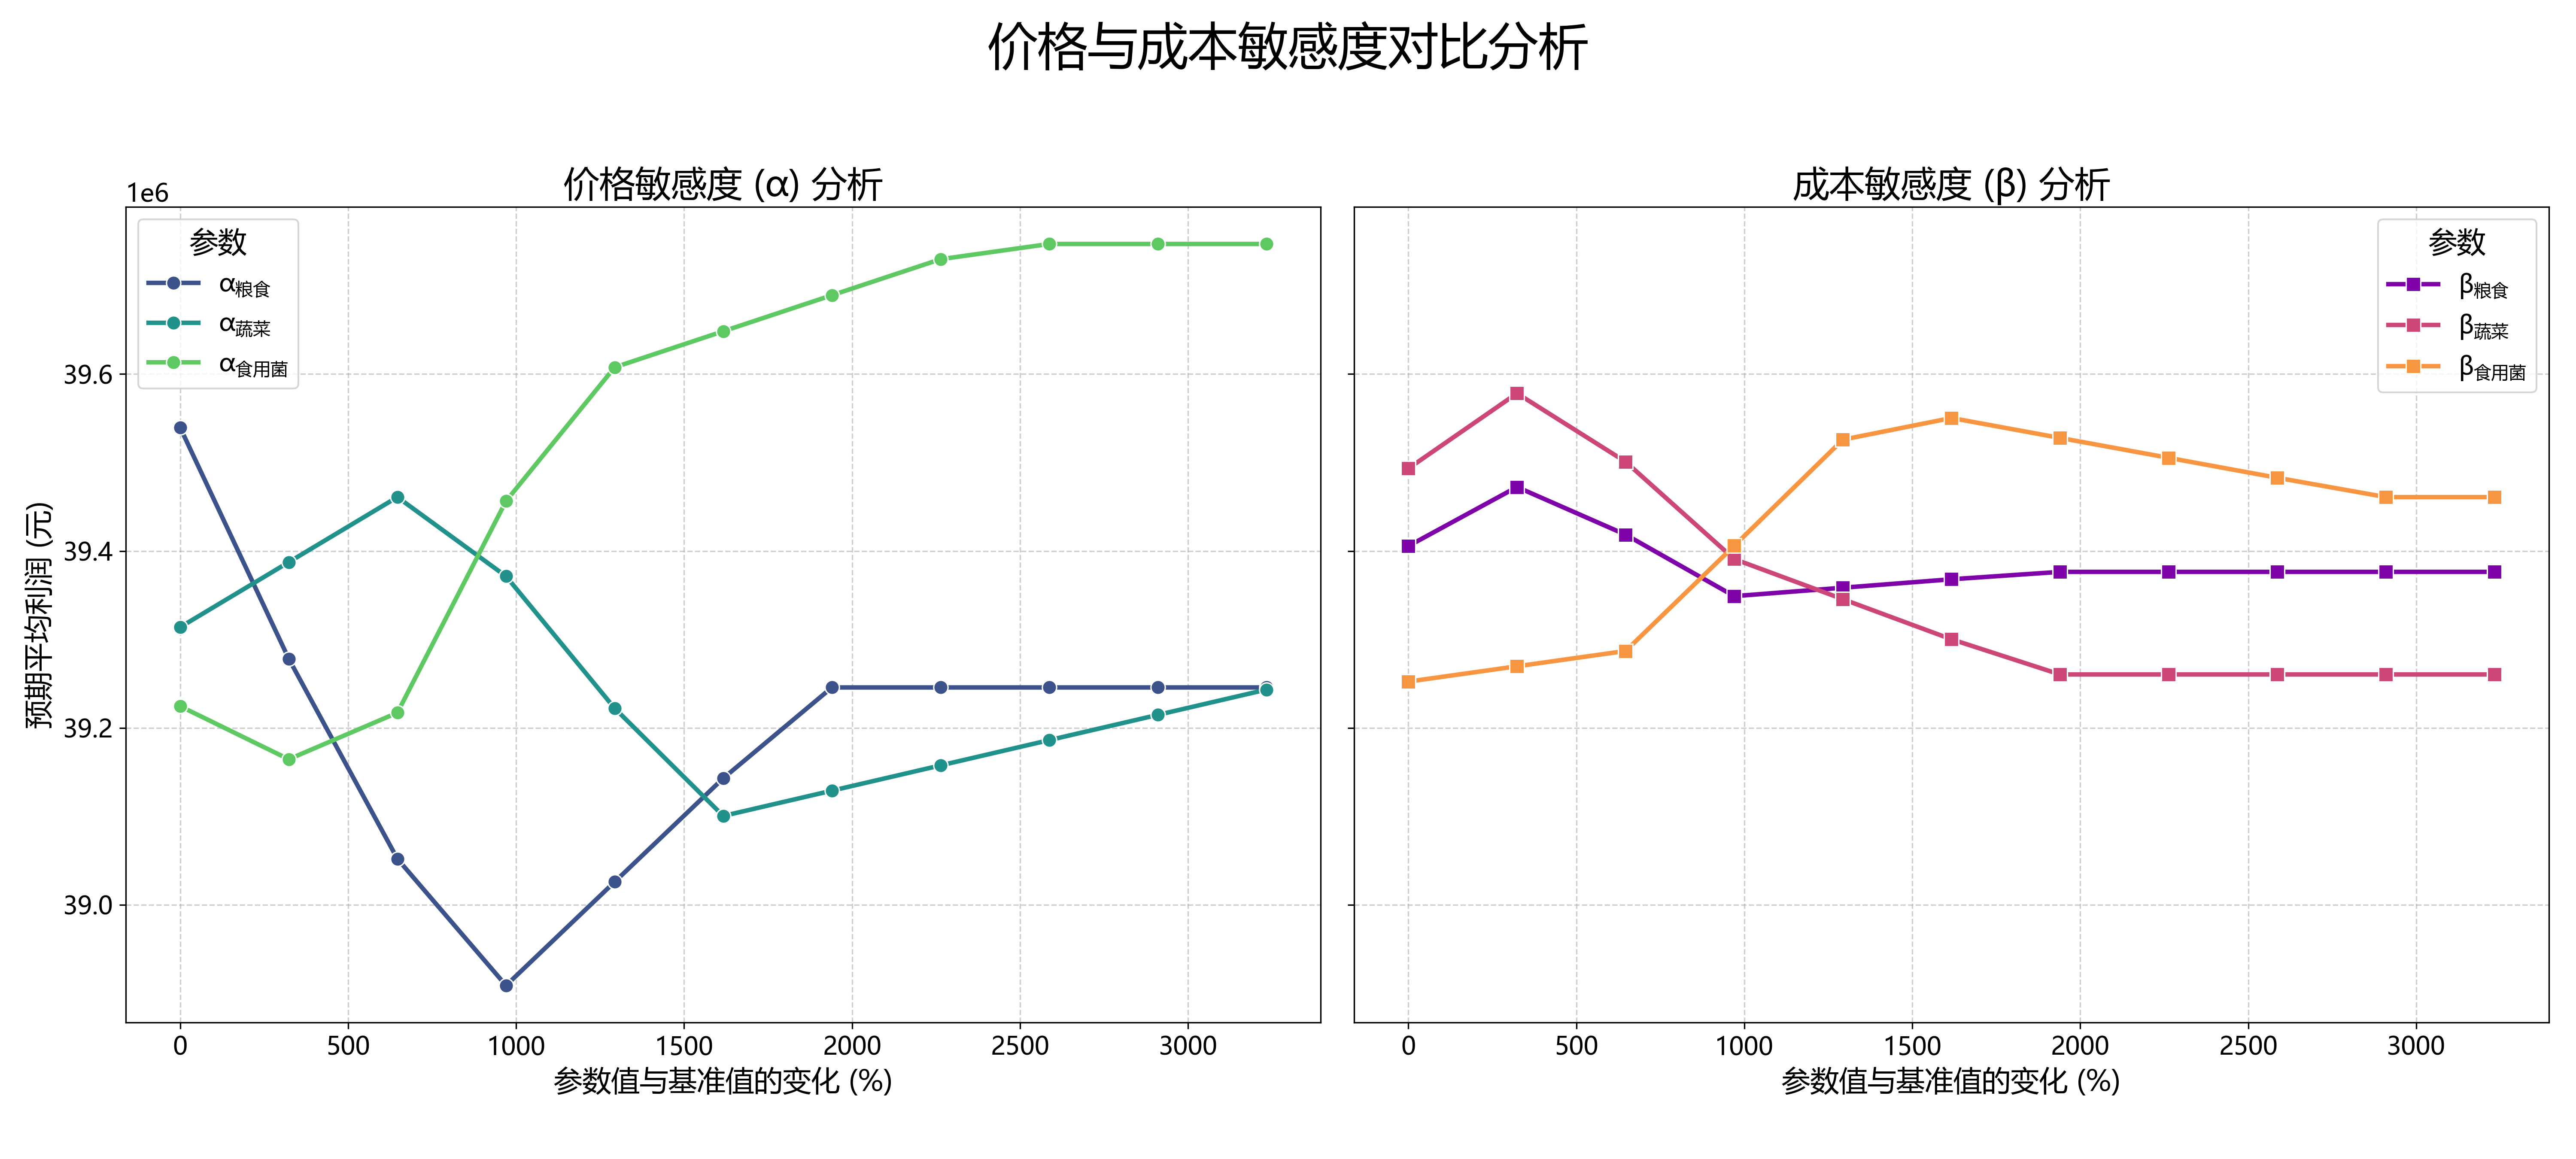
\includegraphics[width=\textwidth]{figs/5问题三/灵敏度分析图.png}
    \caption{预期总利润对六个核心敏感度系数的响应分析。}
    \label{fig:sensitivity_analysis}
\end{figure}

分析结果如图\ref{fig:sensitivity_analysis}所示。可以观察到,预期总利润对食用菌的价格敏感度$p_{\text{fungi}}$变化最为敏感,其对应的曲线斜率最大。这表明,食用菌这类高价值经济作物的市场供需关系是影响该乡村总体经济效益的关键因素。相比之下,总利润对粮食和蔬菜的价格及成本敏感度表现出很强的不敏感性,即使这些参数发生较大变化,最优利润水平也基本保持稳定。这说明,对于大宗农产品,本模型给出的种植策略具有很好的适用性和稳定性。








\newpage

% 参考文献
\bibliographystyle{plain}
\bibliography{reference}
\newpage

\end{document}